% \documentclass[uplatex]{jsreport}
% \usepackage{amssymb,amsthm,amsmath}
% \theoremstyle{definition}
% \renewcommand{\proofname}{\upshape \bfseries 証明}
% \renewcommand{\labelenumi}{(\roman{enumi})}

% \allowdisplaybreaks[1]


\RequirePackage{plautopatch}
\plautopatchdisable{eso-pic} % https://oku.edu.mie-u.ac.jp/tex/mod/forum/discuss.php?d=2956, pdfpages との相性を良くする
\documentclass[12pt,dvipdfmx,uplatex]{jsarticle}
% \documentclass[11pt,autodetect-engine,dvi=dvipdfmx,ja=standard,
% label-section=modern, % モダーン!(Theorem Appendix A.3 みたいなアホがない)
% a4paper]{bxjsarticle}

\input{../../../preamble-j}
% \usepackage[margin=15mm]{geometry}
% \usepackage{geometry}
\usepackage{multirow}
\input{../../../pikachu}
\input{../../../colorsforprint.tex}
\usepackage{pdfpages} % at the final compile, delete the option "demo"
\usepackage[top=10truemm,bottom=15truemm,left=12truemm,right=12truemm]{geometry} %DO NOT option ``a4paper", it changes the size of outputed PDF
% \newtheorem{thm}{定理}[section]
% \newtheorem{lem}[thm]{補題}
% \newtheorem{defi}[thm]{定義}
% \newtheorem{cor}[thm]{系}
% \newtheorem{exam}[thm]{例}
% \newtheorem{rem}[thm]{注意}
% \newtheorem{conj}[thm]{予想}
% \newtheorem{ques}[thm]{問題}


\Crefname{figure}{図}{図}
\crefname{figure}{図}{図}

% \AtBeginEnvironment{thm}{\begin{minipage}{\textwidth}\vspace{1em}}
% \AtEndEnvironment{thm}{\end{minipage}}


\DeclareMathOperator{\ballsub}{\underset{\text{ball}}{\subset}}
\renewcommand{\dx}{\; dx}
\newcommand{\uah}{\underline{\ah}}
\newcommand{\MJ}{MJ}
\newcommand{\img}{\sqrt{-1}}
% \DeclareMathOperator{\MJ}{MJ}

\newcommand{\bigzero}{\mbox{\Large\textbf{0}}}
\newcommand{\rvline}{\hspace*{-\arraycolsep}\vline\hspace*{-\arraycolsep}}
\newcommand\Tstrut{\rule{0pt}{2.6ex}}         % = `top' strut
\newcommand\Bstrut{\rule[-0.9ex]{0pt}{0pt}}   % = `bottom' strut

\makeatletter
\newcommand{\neutralize}[1]{\expandafter\let\csname c@#1\endcsname\count@}
\makeatother

\newenvironment{claimbis}[1]
  {\renewcommand{\thethm}{\ref{#1}$'$}%
   \neutralize{claim}\phantomsection
   \begin{claim}}
  {\end{claim}}

% \begin{align*}
%   \begin{array}{ccc}
%     M & \stackrel{\phi}{\longrightarrow} & M' \\
%     \rotatebox{90}{$\in$} & & \rotatebox{90}{$\in$} \\
%     p & \longmapsto & \phi(p)
%   \end{array}
% \end{align*}

% \begin{figure}[H]
%   \centering
%   \begin{tikzpicture}
%     \node (ef) at (0, 1.2) {$E\times F$};
%     \node (g) at (1.2, 1.2) {$G$};
%     \node (m) at (0, 0) {$M$};
%     \draw[->] (ef) to node[above] {$\scriptstyle b$} (g);
%     \draw[->] (ef) to node[left] {$\scriptstyle \phi$} (m);
%     \draw[->] (m) to node[right] {$\scriptstyle \exists !\tilde{b}$} (g);
%     \node (a) at (0.4, 0.7) {$\scriptstyle \circlearrowleft$};
%   \end{tikzpicture}
% \end{figure}

% \begin{empheq}[left={|x|=\empheqlbrace}]{alignat*=2}
%   x & \quad (x\geq 0) \\
%   -x & \quad (otherwise) 
% \end{empheq}

% easylist
% \ListProperties(Margin2=2em,Space1*=0em,FinalMark={)}, Style2*=\textbullet, Hide2=2)

% inline eqs. w/. numbering
% e.g.
% \inlineequation[eq:matsushima-p191-1]{\forall X\in\ge,\ \ad(X)\circ J = J\circ \ad(X)}

% \begin{figure}[H]
%   \centering
%   %   \raggedleft
%   %   \raggedrightp
%   %   \includegraphics[scale=0.08]{graph/fig1.jpg}
%   \includegraphics[scale=0.08]{graph/fig1-2.jpg}
%   \label{fig:fig1}
% \end{figure}


% % \maketitleの余白を調整
% \makeatletter
% \renewcommand{\@maketitle}{\newpage
%   % \null
%   % \vskip 2em 
%   \begin{center}
%     {\LARGE \@title \par} % \vskip 1.5em
%     {\large \lineskip .5em
%       \begin{tabular}[t]{c}\@author
%       \end{tabular}\par
%     }
%     % \vskip 1em
%     % {\large \@date}
%   \end{center}
%   % \par
%   % \vskip 0.5em
% }
% \makeatother

\usepackage{advdate} % \AdvanceDate[-1]\today の進捗報告,みたいな



\makeatletter
\@addtoreset{equation}{section}
\def\theequation{\thesection.\arabic{equation}}
\makeatother

\begin{document}

\begin{titlepage}
% \newgeometry{top=10truemm,bottom=15truemm,left=12truemm,right=12truemm}
\huge
\centering
{\Huge 2021年度}

\vspace{4cm}

% \raggedright
\begin{center}
  修士論文題目
\end{center}

% \flushleft
\centering
\noindent
\underline{\large Riemann 対称空間上における測地線の簡約部分 Lie 代数への射影に対する有界性}

\underline{\large ---低階数・低次元の場合---}

\vspace{10cm}

\Large
\raggedright
\begin{tabular}{ll}
学生証番号 \quad {} & \underline{45-196010} \\
フリガナ & オクダ タカコ \\
氏名 & \underline{奥田 堯子}
\end{tabular}

\end{titlepage}

\newgeometry{}

\makeatletter

\renewcommand*{\l@section}[2]{%
  \ifnum \c@tocdepth >\z@
    \addpenalty{\@secpenalty}%
    \addvspace{1.0em \@plus\p@}%
    \begingroup
      \parindent\z@
      \rightskip\@tocrmarg
      \parfillskip-\rightskip
      \leavevmode\headfont
      \setlength\@lnumwidth{1.5em}% 元1.5em [2003-03-02]
      \advance\leftskip\@lnumwidth \hskip-\leftskip
      #1\nobreak
      \leaders\hbox{\normalfont$\m@th \mkern \@dotsep mu\hbox{.}\mkern \@dotsep mu$}\hfill %
      \nobreak\hbox to\@pnumwidth{\hss#2}\par
    \endgroup
  \fi}

\makeatother

% {% \hypersetup{linkbordercolor=black}
%   \hypersetup{linkcolor=black}
% % or \hypersetup{linkcolor=black}, if the colorlinks=true option of hyperref is used
% \tableofcontents
% }

\setcounter{tocdepth}{3}
\tableofcontents


\clearpage

\section*{導入}
\addcontentsline{toc}{section}{導入}
$G$を非コンパクトな実半単純Lie群,$K$を$G$の極大コンパクト部分群で$G$のCartan対合$\Theta$に対して$K = \Theta K $なるものとする.$\ge = \ka \oplus \pe $を$\Theta$の微分$d\Theta$による$\ge$のCartan分解とするとき,$G/K$は$\pe$と微分同相である.$G/K$に$\ge$のKilling形式$B$から定まるRiemann計量によってRiemann多様体の構造を定める.$G$の単位元の$G/K$での像$eK$を通る$G/K$の極大測地線は$B(X, X) = 1 $なる$X\in \pe$によって$e^{tX}K $,$t\in \real$と書ける.$H$を$G$の非コンパクトな閉部分群で,$H = \Theta H$を満たすものとし,$\pe$での$B$に対する$\ha\cap \pe$の直交補空間を$\per{\ha}\cap\pe$とする.測地線$e^{tX}K$の$\ha\cap\pe$成分と$\per{\ha}\cap\pe$成分への分解を与える定理として次の定理が知られている.

\begin{thm*}\cite[Lemma~6.1]{kob89}\label{thm:kob89-lem6.1}

  $\pi\colon  (\ha\cap\pe)\oplus (\per{\ha}\cap \pe) \ni (Y, Z)\mapsto e^{Y}e^{Z}K \in G/K $は上への微分同相である.
\end{thm*}
この定理を用いて$X\in \pe$に対し,$(Y(X), Z(X))\defeq \inv{\pi}(e^X\cdot K)\in (\ha\cap\pe)\oplus (\per{\ha}\cap \pe)$と定義すると,任意の$t\in \real$に対して$e^{tX}K = e^{Y(tX)}e^{Z(tX)}K $である.

$G = \SU(1,1) $,$H = \SO(1,1) $とするとき,$t\in \real$に対し,$Y(tX) $は\Cref{fig:y-and-z}に図示するような幾何学的な意味を持つ.\Cref{fig:y-and-z}は{\Poincare}円板における測地線$e^{tX}K$ (赤色の斜め線) とその上の一点$e^{tX}K$から$eK$の$H$軌道 (中央の直線) に下ろした垂線の足 (緑の丸) が$e^{Y(tX)}K $である.
\begin{figure}[H]
  \centering
  %   \raggedleft
  %   \raggedrightp
  %   \includegraphics[scale=0.08]{graph/fig1.jpg}
  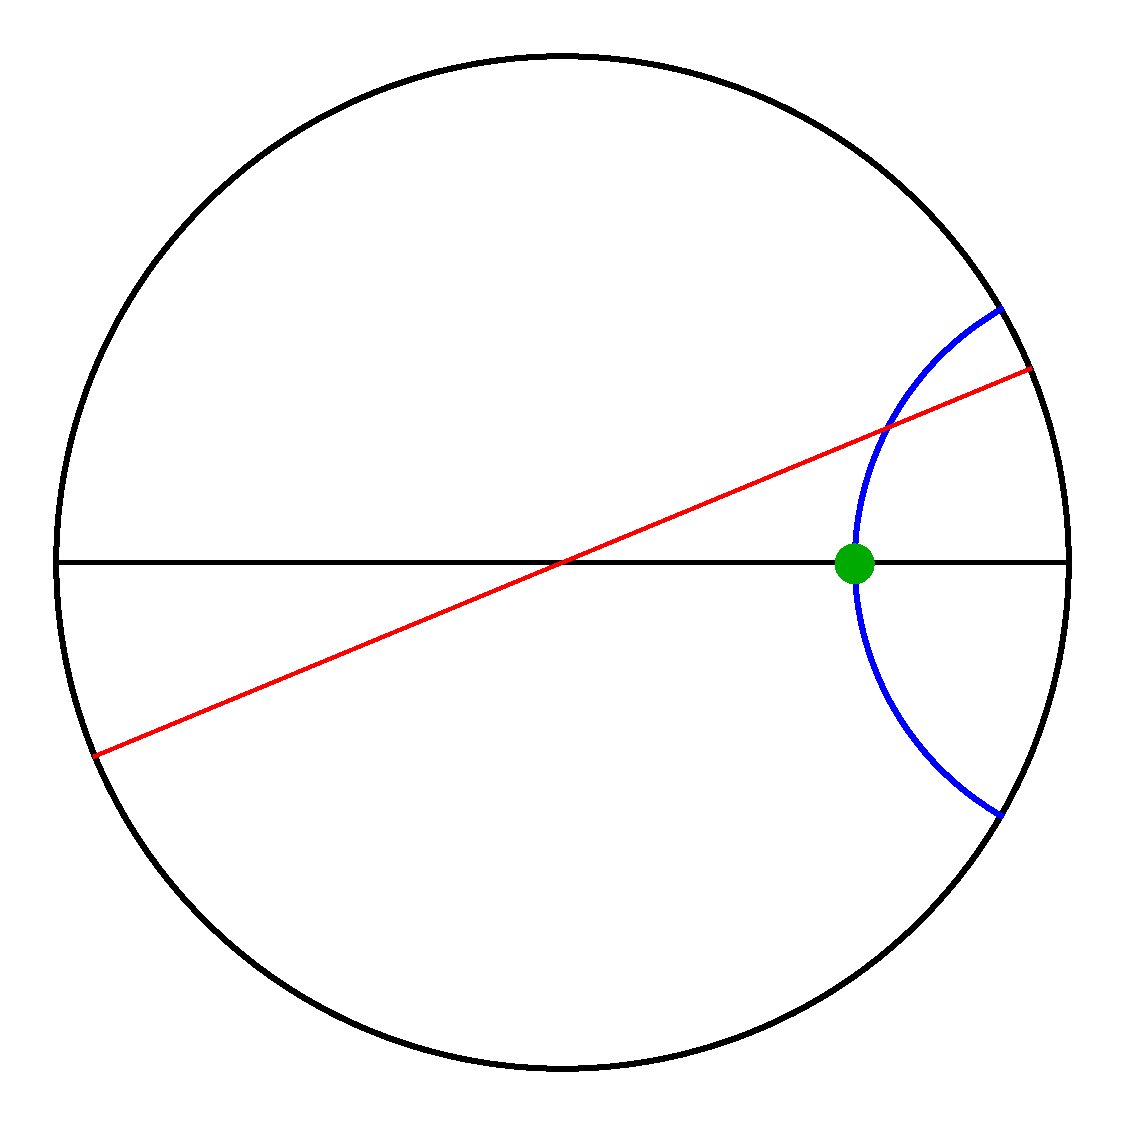
\includegraphics[scale=0.3]{../graph/y-and-z.pdf}
  \caption{{\Poincare}円板における$Y(tX) $の幾何学的意味}
  \label{fig:y-and-z}
\end{figure}

本論文では小林俊行氏による次の予想について考察し,$G$が実階数1の場合の肯定的な結果を得た.
\begin{yosou*}
    $Y(\real X)$は$ \ha\cap \pe$の有界な部分集合である$ \iff   [X_1, X_2]\neq 0 $であるか$X_1 = 0$である.

  ただし$X = X_1 + X_2 $はベクトル空間としての分解$\pe =(\pe\cap \ha)\oplus(\pe\cap\per{\ha}) $に対応する$X\in \pe$の分解とする.
\end{yosou*}

% \begin{thm*}
%   $G$が実階数1のとき,$Y(\real X) $が有界であることと$X=0$または$X\in \pe\setminus\ha$であることが同値である.
% \end{thm*}

\section*{謝辞}
\addcontentsline{toc}{section}{謝辞}

% 本研究および修士課程全体において常に洞察に富むご助言と丁寧なご指導を賜った指導教員の小林俊行教授に深謝の意を表する.% 小林先生のご指導なしには本論文はあり得なかった.
また,文献の情報から数学的な議論にわたり様々なご助言をくださった,修了生も含む小林研究室のみなさまにも心より感謝する.特に小林研究室の田内大渡氏には幾度も議論いただいたことに御礼申し上げたい.

最後に,学部時代からセミナーに付き合ってくださり,ときに精神的にも支えてくださった友人に,特に近藤彪生氏には同じ「修士3年生」として修士論文の締め切り前に多大な励ましをいただいたことに感謝の意を表して謝辞とする.


\clearpage

\section{設定と$\ha$射影の基本的な性質,\Cref{yosou:1121}の観察}
%%% Local Variables:
%%% mode: japanese-latex
%%% TeX-engine: uptex
%%% TeX-master: "okuda-master-thesis"
%%% TeX-PDF-mode: t
%%% TeX-PDF-from-DVI: "Dvipdfmx"
%%% End:

\subsection{記号の設定}
本論文の基本的な設定は次のとおりであり,この他に必要な条件は都度明示することとする.

\begin{nttdef}
  \leavevmode\vspace{-1em}
  \begin{itemize}
  \item $\nat,\real, \cpx,\quat$をそれぞれ0を含む自然数全体,実数全体,複素数全体,四元数全体の集合とする.
  \item $G$を非コンパクト実簡約Lie 群,$H$を$G$の非コンパクトかつ連結成分有限個の閉部分群で,$G$のCartan対合$\Theta$に対して$\Theta H = H$なるものとする.
  \item $\ge \defeq \Lie G,\; \ha \defeq \Lie H$とし,$\ge = \ka\oplus \pe$を $\theta \defeq d\Theta$ によるCartan分解とする.
  \item $\ze(\ha)\defeq \{Y\in \ha\mid [Y,\ha] = \{0\} \} $とする.
  \item $e$を$G$の単位元とし,$o_K \defeq eK\in G/K$とする.
  \item $\lyama{-},{-} \ryama$を,$\ge$上の$G$-不変な非退化対称双線型形式で,$\ka$上負定値,$\pe$上正定値で$\ka\perp \pe$なるものとする.
  \item $\per{\ha}\ \defeq \{W\in \ge\mid \lyama W, \ha\ryama = \{0\}\} $とする.
  \item $X\in \pe$に対し,ベクトル空間としての分解$\pe =( \ha\cap \pe)\oplus(\per{\ha}\cap \pe) $に対応した分解を$X = X_1 + X_2 $,$X_1 \in \ha\cap \pe$,$X_2\in \per{\ha}\cap \pe$とする.
  \item $(M,d_M)$を$M$の上の任意の2点に対し一意的な測地線が存在するRiemann多様体と$M$上の計量から定まる距離とする.相異なる点$p,q,r \in M$に対し,
    \begin{itemize}
    \item $\gamma_{p,q}\colon [0, d_{M}(p,q)] \to M$を,$\gamma(0) =  p$,$\gamma(d_{M}(p,q)) = q $なる測地線とする.
    \item $\measuredangle_{p}(q, r)$を$\gamma_{p,q} $と$\gamma_{p,r} $が$p$においてなす角とする.
    \end{itemize}
  \end{itemize}  
\end{nttdef}

以下の\Cref{thm:kob89-lem6.1}を用いて,$X\in \pe$に対し,
\begin{align*}
{(Y(X), Z(X))\defeq \inv{\pi}(e^X\cdot o_K)\in (\ha\cap\pe)\oplus (\per{\ha}\cap \pe)}
\end{align*}
と定義する.
\begin{thm}(\cite[Lemma~6.1]{kob89})\label{thm:kob89-lem6.1}
  \begin{align*}
    \pi\colon  (\ha\cap\pe)\oplus (\per{\ha}\cap \pe) \ni (Y, Z)\mapsto e^{Y}e^{Z}\cdot o_K \in G/K
  \end{align*}
  は上への微分同相である.
\end{thm}


ここで,$Y(\real X) $の有界性について,次の\Cref{prob:1121}が小林俊行氏によって提起された.


\begin{prob}(小林俊行氏による)\label{prob:1121}
  ${\pe_{H,\bdd}\defeq \{X\in \pe\mid Y(\real X)\text{ が } \ha\cap \pe \text{ の有界集合である.}  \}}  $と定めるとき,
  \begin{enumerate}
  \item $G$が実半単純Lie群ならば$\pe\setminus\pe_{H,\bdd} $は測度0であるか?
  \item \begin{align}
          \pe_{H,\bdd} = {(\per{\ha}\cap\pe) \cup \{X\in \pe\mid  [X_1, X_2]\neq 0 \text{ かつ }\pe\cap \ze_{\ze(\ha)}(X)  = \{0\} \text{ である.} \}} \label{eq:prob-1121}
        \end{align}
        となっているか?
      \end{enumerate}
\end{prob}

\Cref{prob:1121}についての基本的な事項を挙げる.

\begin{lem}\label{lem:basic-prob}
  \leavevmode\vspace{-1em}
  \begin{enumerate}
  \item \Cref{prob:1121}において,2が成り立つならば1が成り立つ.
  \item ${\pe_{H,\bdd} \subset (\per{\ha}\cap\pe) \cup \{X\in \pe\mid  [X_1, X_2]\neq 0 \text{ かつ }\pe\cap \ze_{\ze(\ha)}(X) = \{0\}  \text{ である.} \}}$が成り立つ.
  \item $X \in \pe $が$X_1 = 0$を満たすならば$X\in \pe_{H,\bdd} $である.
  % \item 1,2より\Cref{prob:1121}と「$X\in \pe$が$[X_1,X_2]\neq 0$ならば$X\in \pe_{H,\bdd} $である」は同値である.
  \item $G$が実階数1ならば,\Cref{eq:prob-1121}と「$\pe_{H,\bdd} =  \{0\}\cup \pe\setminus\ha $」は同値である.
  \end{enumerate}
\end{lem}

\begin{npfwn}[\Cref{lem:basic-prob}]
  \leavevmode\vspace{-1em}
  \begin{enumerate}
  \item \redtext{次が測度0であることを示せば十分である.}\footnote{示せていません.}
    \begin{align*}
      & \pe\setminus \{X\in \pe\mid  [X_1, X_2]\neq 0 \text{ かつ }\pe\cap \ze_{\ze(\ha)}(X)  = \{0\} \text{ である.} \}\\
      =&\ \{X\in \pe\mid  [X_1, X_2] = 0 \text{ または }\pe\cap \ze_{\ze(\ha)}(X)  \neq \{0\} \text{ である.} \}
    \end{align*}
    まず,$\{X\in \pe\mid  [X_1, X_2] = 0\}$と$X\in  \ze_{\pe}(X_1) $は同値である.$\ze_{\pe}(X_1) = \{W\in \pe\mid [X_1,W] = 0  \} $

    $\{X\in \pe\mid \pe\cap \ze_{\ze(\ha)}(X)  \neq \{0\} \text{ である.}\} $は$\{0\}\subsetneq \ze(\ha)\cap\pe$を含む極大分裂可換部分代数を$\ah$とするとき,
    
  \item $X\nin\per{\ha}\cap \pe $なる$X\in \pe$に対し,$[X_1,X_2] = 0$ならば$e^{tX_1}e^{tX_2}\cdot o_K = e^{t(X_1 + X_2)}\cdot o_K = e^{tX}\cdot o_K$である.したがって\Cref{thm:kob89-lem6.1}より$Y(tX) = tX_1 $,$Z(tX) = tX_2 $であることから$Y(\real X) = \real X_1 $となり,$X_1\neq 0$より$Y(\real X)$は有界集合とならない.

    \redtext{$X\nin\per{\ha}$かつ$ \ze_{\ze(\ha)}(X) \neq \{0\} $の場合に$X\nin \pe_{H,\bdd} $であることが示せていません.}
  \item $X_1 = 0$であることと$ X\in \per{\ha}\cap\pe $であることが同値であることから従う.
  \item $G$が実階数1として次を示せばよい.
    \begin{align}
      \{0\}\cup \pe\setminus \ha = (\per{\ha}\cap\pe) \cup \{X\in \pe\mid  [X_1, X_2]\neq 0 \text{ かつ } \pe\cap \ze_{\ze(\ha)}(X) = \{0\}  \text{ である.} \}\label{eq:basic-prob}
    \end{align}
    $G$の実階数が1かつ$H$が非コンパクトであるから$\ha\cap\pe$は極大分裂可換部分代数であり,右辺の2つ目の集合は$\ze(\ha)\cap\pe \subset \real X_{1}\neq \{0\} $より$\{X\in \pe\mid  [X_1, X_2]\neq 0 \}$となる.よって\Cref{eq:basic-prob}の右辺は$\{X\in \pe\mid X_1 = 0\text{ または }  [X_1, X_2]\neq 0 \text{ である.} \}$と同値である.この集合はさらに$X\in \{0\}\cup\pe\setminus\{0\} $と同値であるから\Cref{eq:basic-prob}が示された.
  \end{enumerate}  
\end{npfwn}

$Y(\real X) $の有界性は$\Ad(k) $-不変である.具体的には\Cref{lem:1101}が成り立つ.
\begin{lem}\label{lem:1101}
  $k\in K$,$X\in \pe$に対し,$X'\defeq \Ad(k)X $,$\ha'\defeq \Ad(k)\ha $とする.$Y'(X'), Z'(X') $を,微分同相$\pi'\colon (\ha'\cap \pe)\oplus (\per{\ha'}\cap \pe)\ni (Y',Z')\mapsto e^{Y'}e^{Z'}\cdot o_K  $を用いて,$X'\in \pe$に対し,$(Y'(X'), Z'(X')) = \inv{\pi'}(e^{X'}\cdot o_K) $と定める.

  このとき$Y(\real X)$が有界であることと$ Y'(\real X') $が有界であることは同値である.
\end{lem}

\begin{npfwn}[\Cref{lem:1101}]
  主張は$(X,\ha) $と$(X',\ha')$に対して対称的であるから,$Y(\real X) $が有界ならば$Y'(\real X') $が有界であることのみを示せば十分である.

  任意に$r\in \real$を取る.$e^{rX'}\cdot o_K = e^{Y'(r X')}e^{Z'(r X')}\cdot o_K  $であり,両辺に左から$\inv{k} $を掛けると,$e^{r X} = e^{\Ad(\inv{k})( Y'(r X'))}e^{\Ad(\inv{k})( Z'(r X'))}\cdot o_K  $を得る.ここで$Y'(rX')\in \ha'\cap \pe $,$Z'(r X')\in \per{\ha'}\cap \pe $であるから$\Ad(\inv{k})(Y'(r X'))\in \ha\cap \pe $,$\Ad(\inv{k})(Z'(r X')) \in \per{\ha}\cap \pe $である.

  \Cref{thm:kob89-lem6.1}により$\pi$は微分同相であるから,任意の$r\in \real$に対して$\Ad(\inv{k})(Y'(r X')) = Y(rX)  $である.$Y'(\real X) = \Ad(k)(Y(\real X))  $であり,$\Ad(k) $は有限次元空間の間の線型写像であるから有界性を保つ.

  以上から\Cref{lem:1101}が示された.  
\end{npfwn}


$Y(\real X) $の有界性を判定しようとする\Cref{prob:1121}と比較して$Z(\real X) $の有界性については次の定理が知られており,有界性の判定はLie環の言葉のみで行える.

\begin{thm}(\cite[Lemmma~5.4]{kob97})\label{thm:kob97}
  $X\in \pe$に対し,$\norm{Z(X)}\geq \norm{X} \sin\phi(X, \ha\cap\pe)$である.ここに$\phi(X,\ha\cap \pe) $は$X$と$\ha\cap \pe$の0でない元がなす角度の最小値${0\leq \phi(X,\ha\cap \pe) \leq \frac{\pi}{2}} $であり,$X\in \pe\setminus \ha $と$ \phi(X,\ha\cap \pe)\neq 0 $は同値である.
\end{thm}

\Cref{thm:kob97}より,$X\in \ha $と$Z(\real X) $が有界であることが同値である.


\subsection{\Cref{prob:1121}の観察: $G = \SU(1,1) $,$H = \SO(1,1) $の場合}

$G = \SU(1,1) $,$H = \SO(1,1) \defeq\lbig\{
\begin{pmatrix}
  \cosh t & \sinh t\\ \sinh t & \cosh t
\end{pmatrix}
\relmiddle| t\in \real \rbig\} $の場合に\Cref{prob:1121}が正しいことは直接計算により確かめられる.

\begin{prop}\label{prop:prob-eg}
  $G = \SU(1,1) $,$H = \SO(1,1) $のとき\Cref{prob:1121}は正しい.
\end{prop}

% \bluetext{$\sulie(1,1) $のKilling形式と$r = \tanh t$の関係を明記せよ.}

\begin{lem}\label{lem:riem-metric-su11}
  $\ge\defeq \sulie(1,1)$のKilling形式から定まる{\Poincare}円板${G/K =\{x+\sqrt{-1}y\mid  x^2 + y^2 < 1 \} }$の計量は$ \dfrac{8(dx^2 + dy^2)}{(1 - x^2 - y^2)^2} $である.
\end{lem}

\begin{npfwn}[\Cref{lem:riem-metric-su11}]
  
  $\ge$の元を$G/K$上の左不変ベクトル場と同一視すると
  \begin{align*}
    X' &\defeq 
         \begin{pmatrix}
           0 & 1 \\ 1 & 0
         \end{pmatrix} = \dfrac{\del}{\del x},\\
    Y' &\defeq 
         \begin{pmatrix}
           0 & \sqrt{-1} \\ -\sqrt{-1} & 0
         \end{pmatrix} = \dfrac{\del}{\del y}
  \end{align*}
  である.$\ge$のKilling形式$B$から定まる$\pe$上のノルム$\norm{-} $に対して$\norm{X'}^2 = \norm{Y'}^2 = 8 $,$B(X', Y' ) = 0$であって,$0\in G/K =\{x+\sqrt{-1}y\mid x^2 + y^2 < 1 \}  $で主張が成り立つ.

  したがって$k_{\theta} \defeq \diag(e^{\sqrt{-1}\theta},e^{-\sqrt{-1}\theta}) $,$a_r\defeq
  \begin{pmatrix}
    \cosh r & \sinh r \\  \sinh r & \cosh r
  \end{pmatrix}
  $とすると,
  \begin{align*}
    &g(d\tau(k_{\theta/2}a_r)(d\tau(k_{-\theta/2})X'), d\tau(k_{\theta/2}a_r)(d\tau(k_{-\theta/2})X')) \\
    =&\ g (d\tau(k_{\theta/2}a_r)(d\tau(k_{-\theta/2})Y'), d\tau(k_{\theta/2}a_r)(d\tau(k_{-\theta/2})Y')) \\
    =&\ 8, \\
    &g(d\tau(k_{\theta/2}a_r)(d\tau(k_{-\theta/2})X'), d\tau(k_{\theta/2}a_r)(d\tau(k_{-\theta/2})Y'))  = 0
  \end{align*}
  なるような計量$g $がKilling形式から誘導される計量であるが,それが主張の形であることを示せば良い (これらのベクトルが何を表しているかは\Cref{fig:riem-metric-su11}参照).

  \begin{figure}[H]
    \centering
    % \raggedleft
    % \raggedrightp
    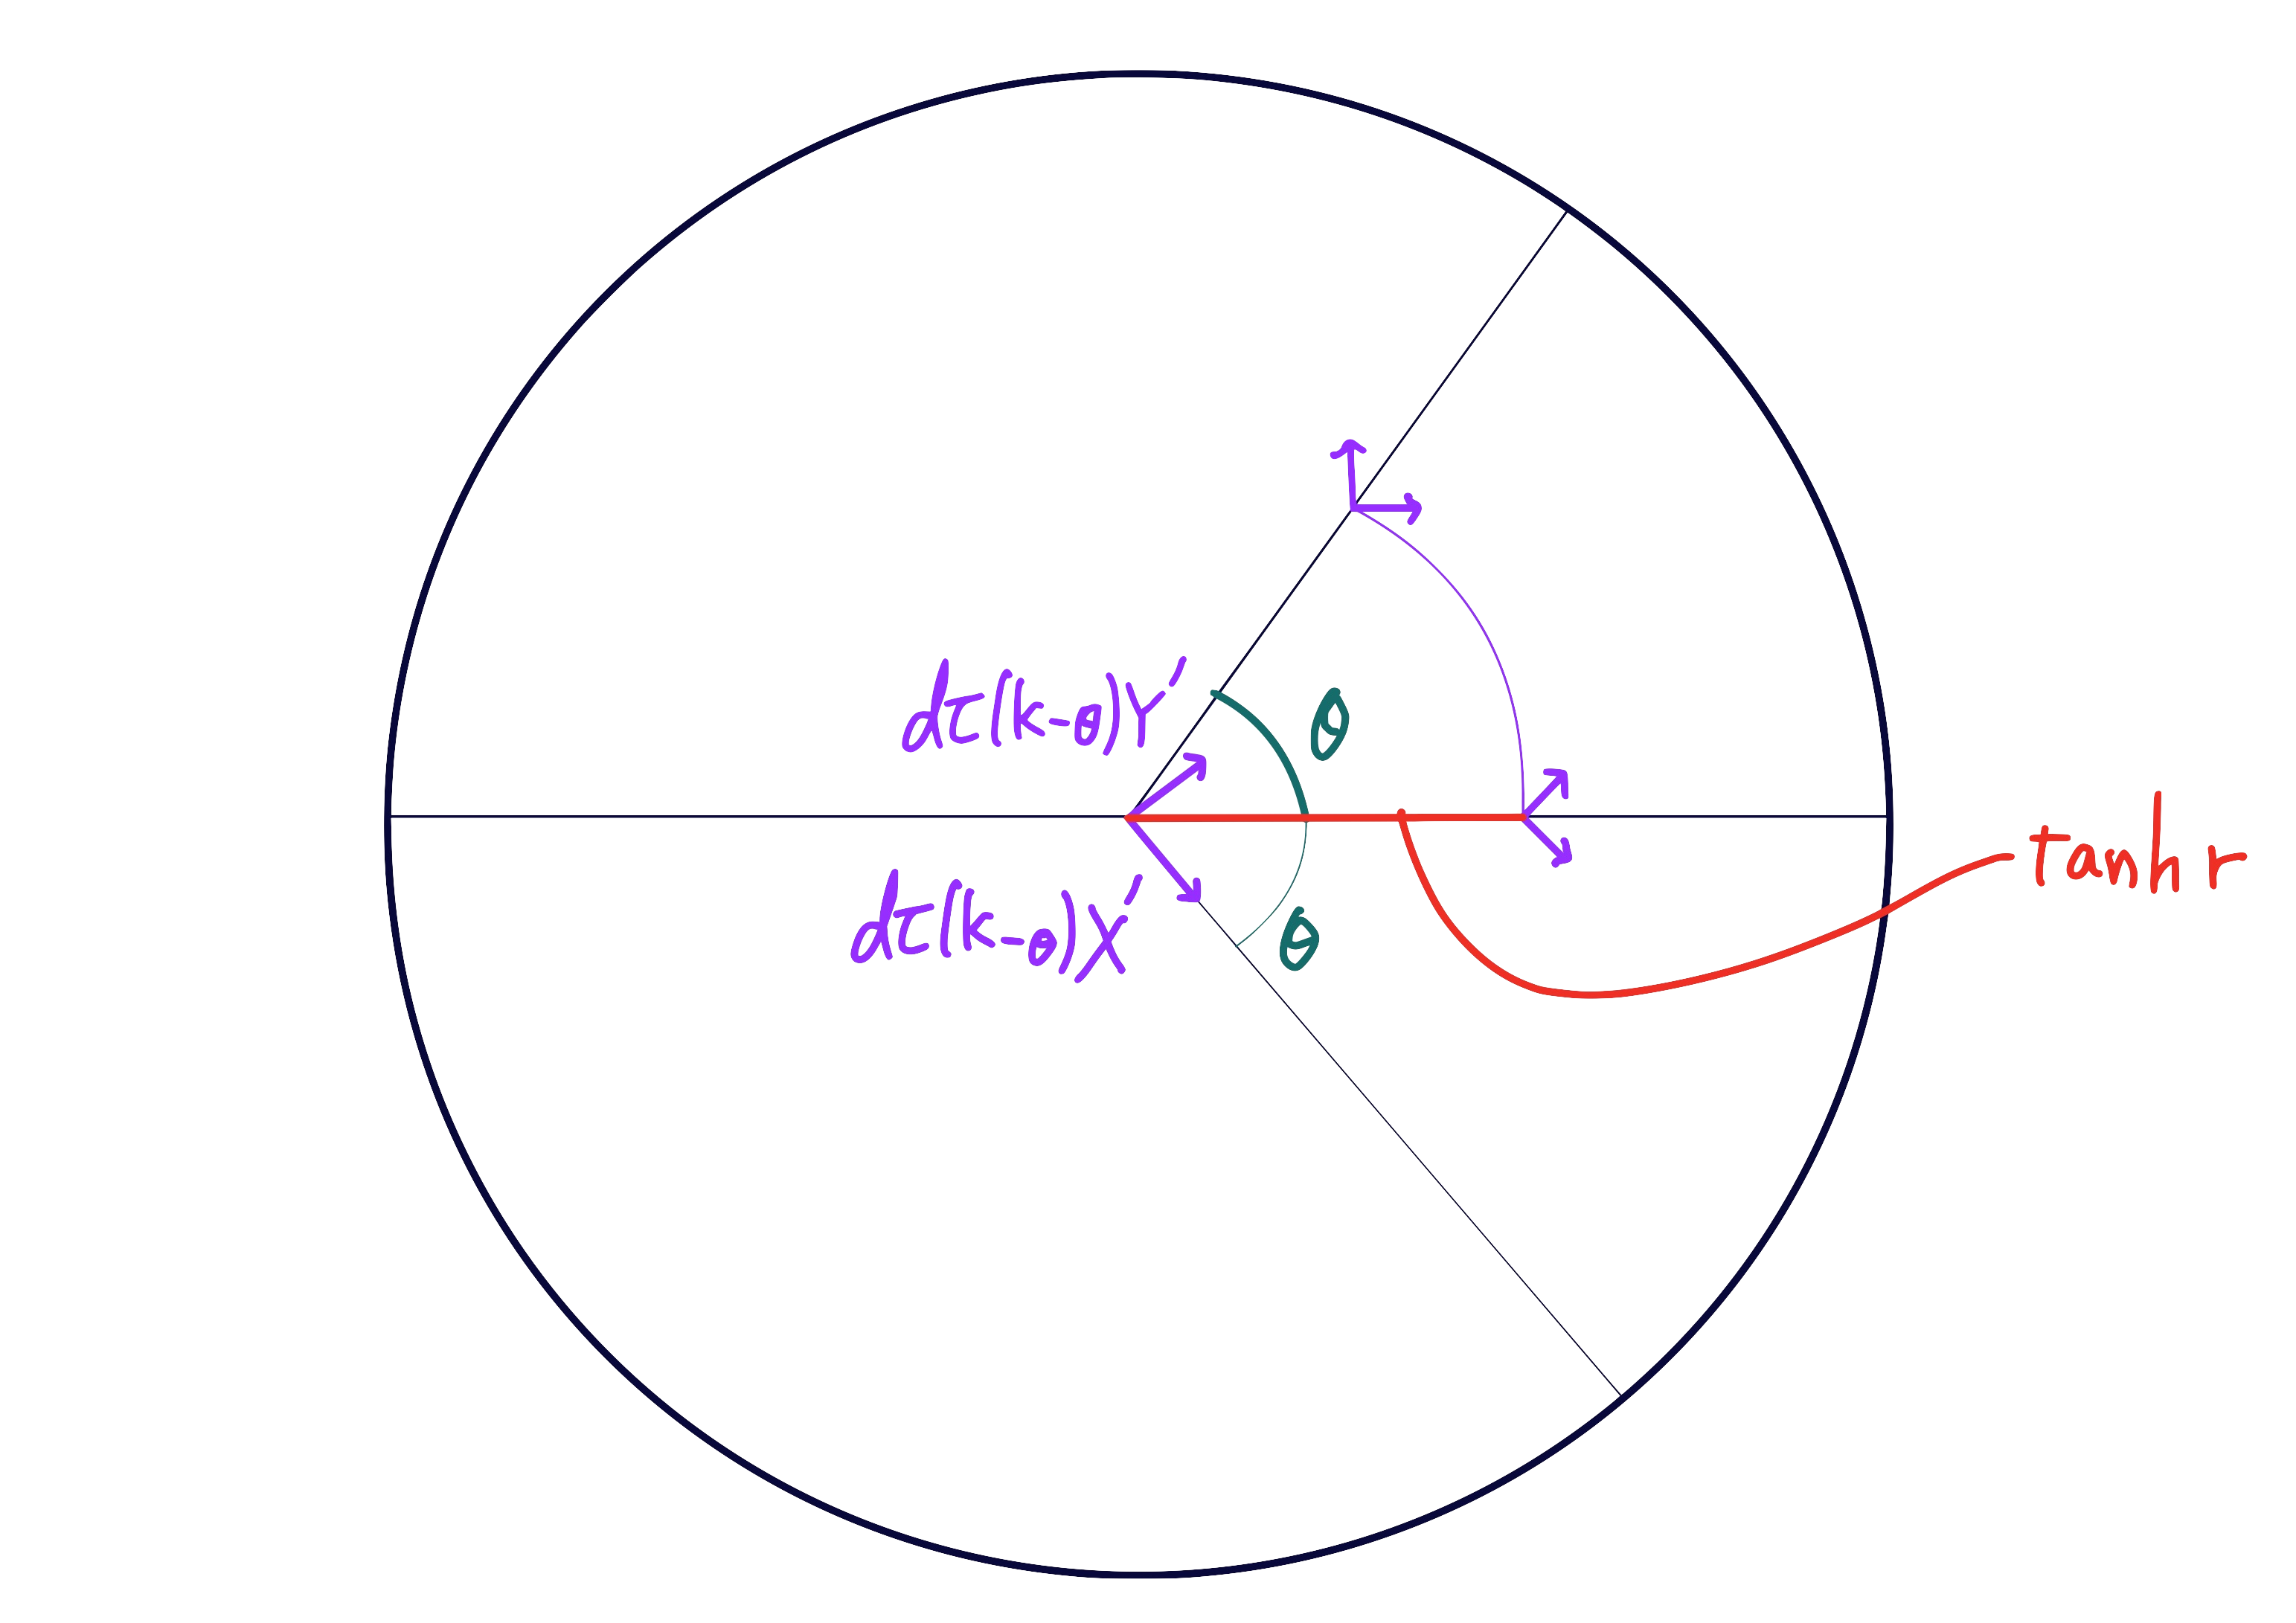
\includegraphics[scale=0.08]{../graph/riem-su11.png}
    % 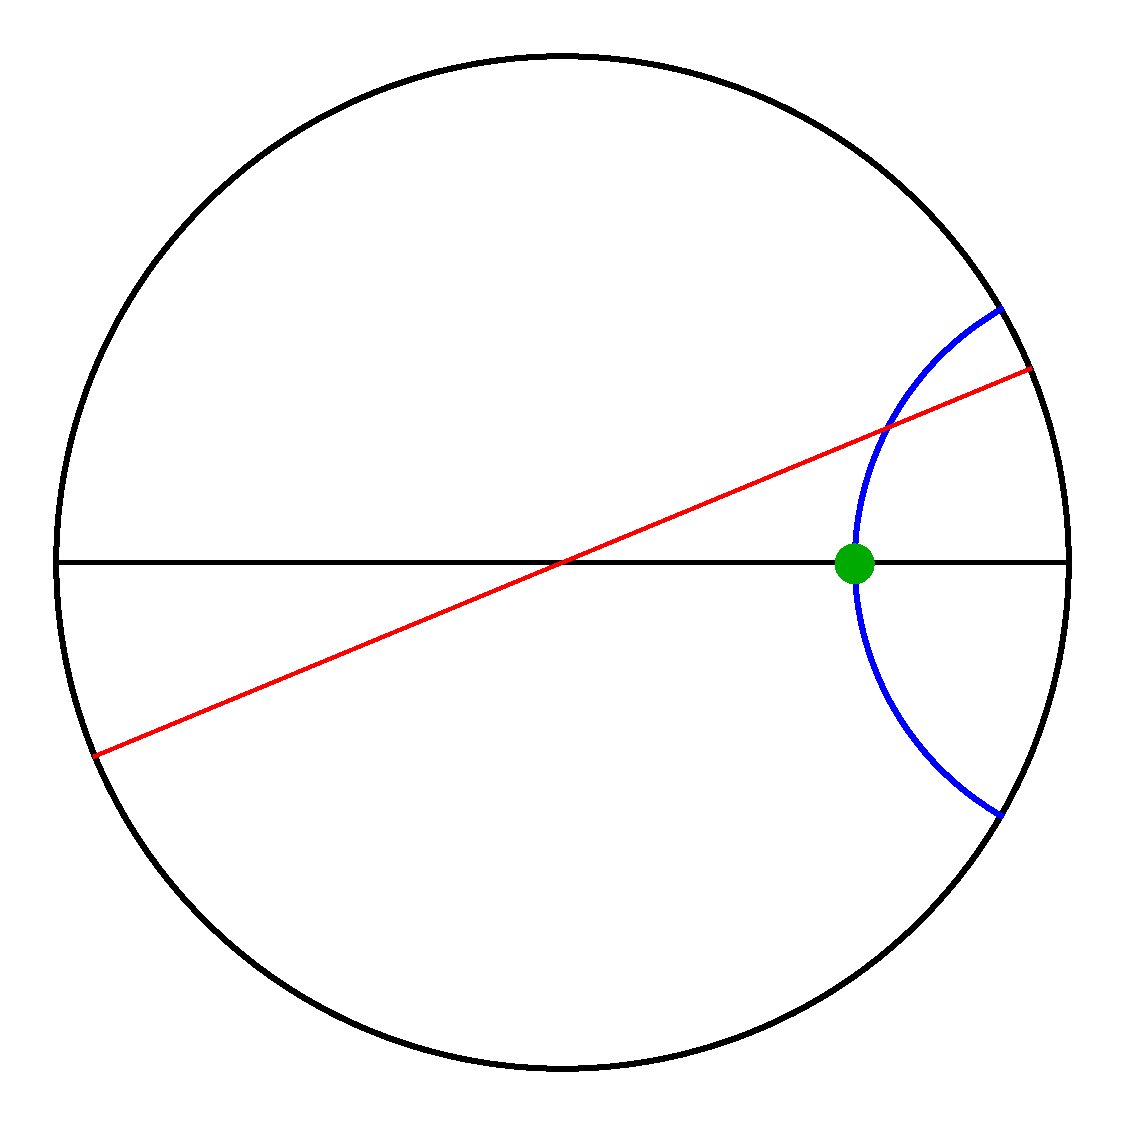
\includegraphics[scale=0.3]{../graph/y-and-z.pdf}
    \caption{}
    \label{fig:riem-metric-su11}
  \end{figure}


  $t = 0$での接ベクトルが$d\tau(k_{\theta/2}a_r)d\tau(k_{-\theta/2})X'$を与える曲線は
  \begin{align*}
    \gamma_x(t) \defeq  e^{\sqrt{-1} \theta}\dfrac{\cosh r\cdot e^{-\sqrt{-1}\theta} \tanh t + \sinh r }{\sinh r\cdot e^{-\sqrt{-1}\theta} \tanh t + \cosh r}
  \end{align*}
  であるから,
  \begin{align*}
    \lbig.\dfrac{d}{dt}\rbig|_{t=0}\gamma_x(t) = d\tau(k_{\theta/2}a_r)d\tau(k_{-\theta/2})X' = (1 - \tanh^2 r)\dfrac{\del}{\del x} = (1-x^2-y^2)\dfrac{\del}{\del x}
  \end{align*}
  である.

  同様に$t = 0$での接ベクトルが$d\tau(k_{\theta/2}a_r)d\tau(k_{-\theta/2})Y'$を与える曲線は
  \begin{align*}
    \gamma_y(t) \defeq  e^{\sqrt{-1} \theta}\dfrac{\cosh r\cdot e^{-\sqrt{-1}\theta}\sqrt{-1} \tanh t + \sinh r }{\sinh r\cdot e^{-\sqrt{-1}\theta}\sqrt{-1} \tanh t + \cosh r}
  \end{align*}
  であるから,
  \begin{align*}
    \lbig.\dfrac{d}{dt}\rbig|_{t=0}\gamma_y(t) = d\tau(k_{\theta/2}a_r)d\tau(k_{-\theta/2})Y' = (1 - \tanh^2 r)\dfrac{\del}{\del y} = (1-x^2-y^2)\dfrac{\del}{\del y}
  \end{align*}
  である.

  以上より$g  =  \dfrac{8(dx^2 + dy^2)}{(1 - x^2 - y^2)^2} $が示された.
\end{npfwn}


\begin{npfwn}[\Cref{prop:prob-eg}]


  $k_{\theta} \defeq \diag(e^{\sqrt{-1}\theta},e^{-\sqrt{-1}\theta}) $,$X_{\theta} \defeq k_{\theta/2}
  \begin{pmatrix}
    0 & 1 \\ 1 & 0
  \end{pmatrix}
  k_{-\theta/2}$とすると,$\pe\setminus\{0\} =  \{tX_{\theta}\mid t\in \real_{>0},\ 0\leq \theta\leq \pi\}$である.この$X_{\theta} $と$t\in \real$に対して$Y(tX_{\theta} ) = s
  \begin{pmatrix}
    0 & 1 \\ 1 & 0
  \end{pmatrix}
  $なる$s\in \real $を求める.


  
  \begin{figure}[H]
    \centering
    % \raggedleft
    % \raggedrightp
    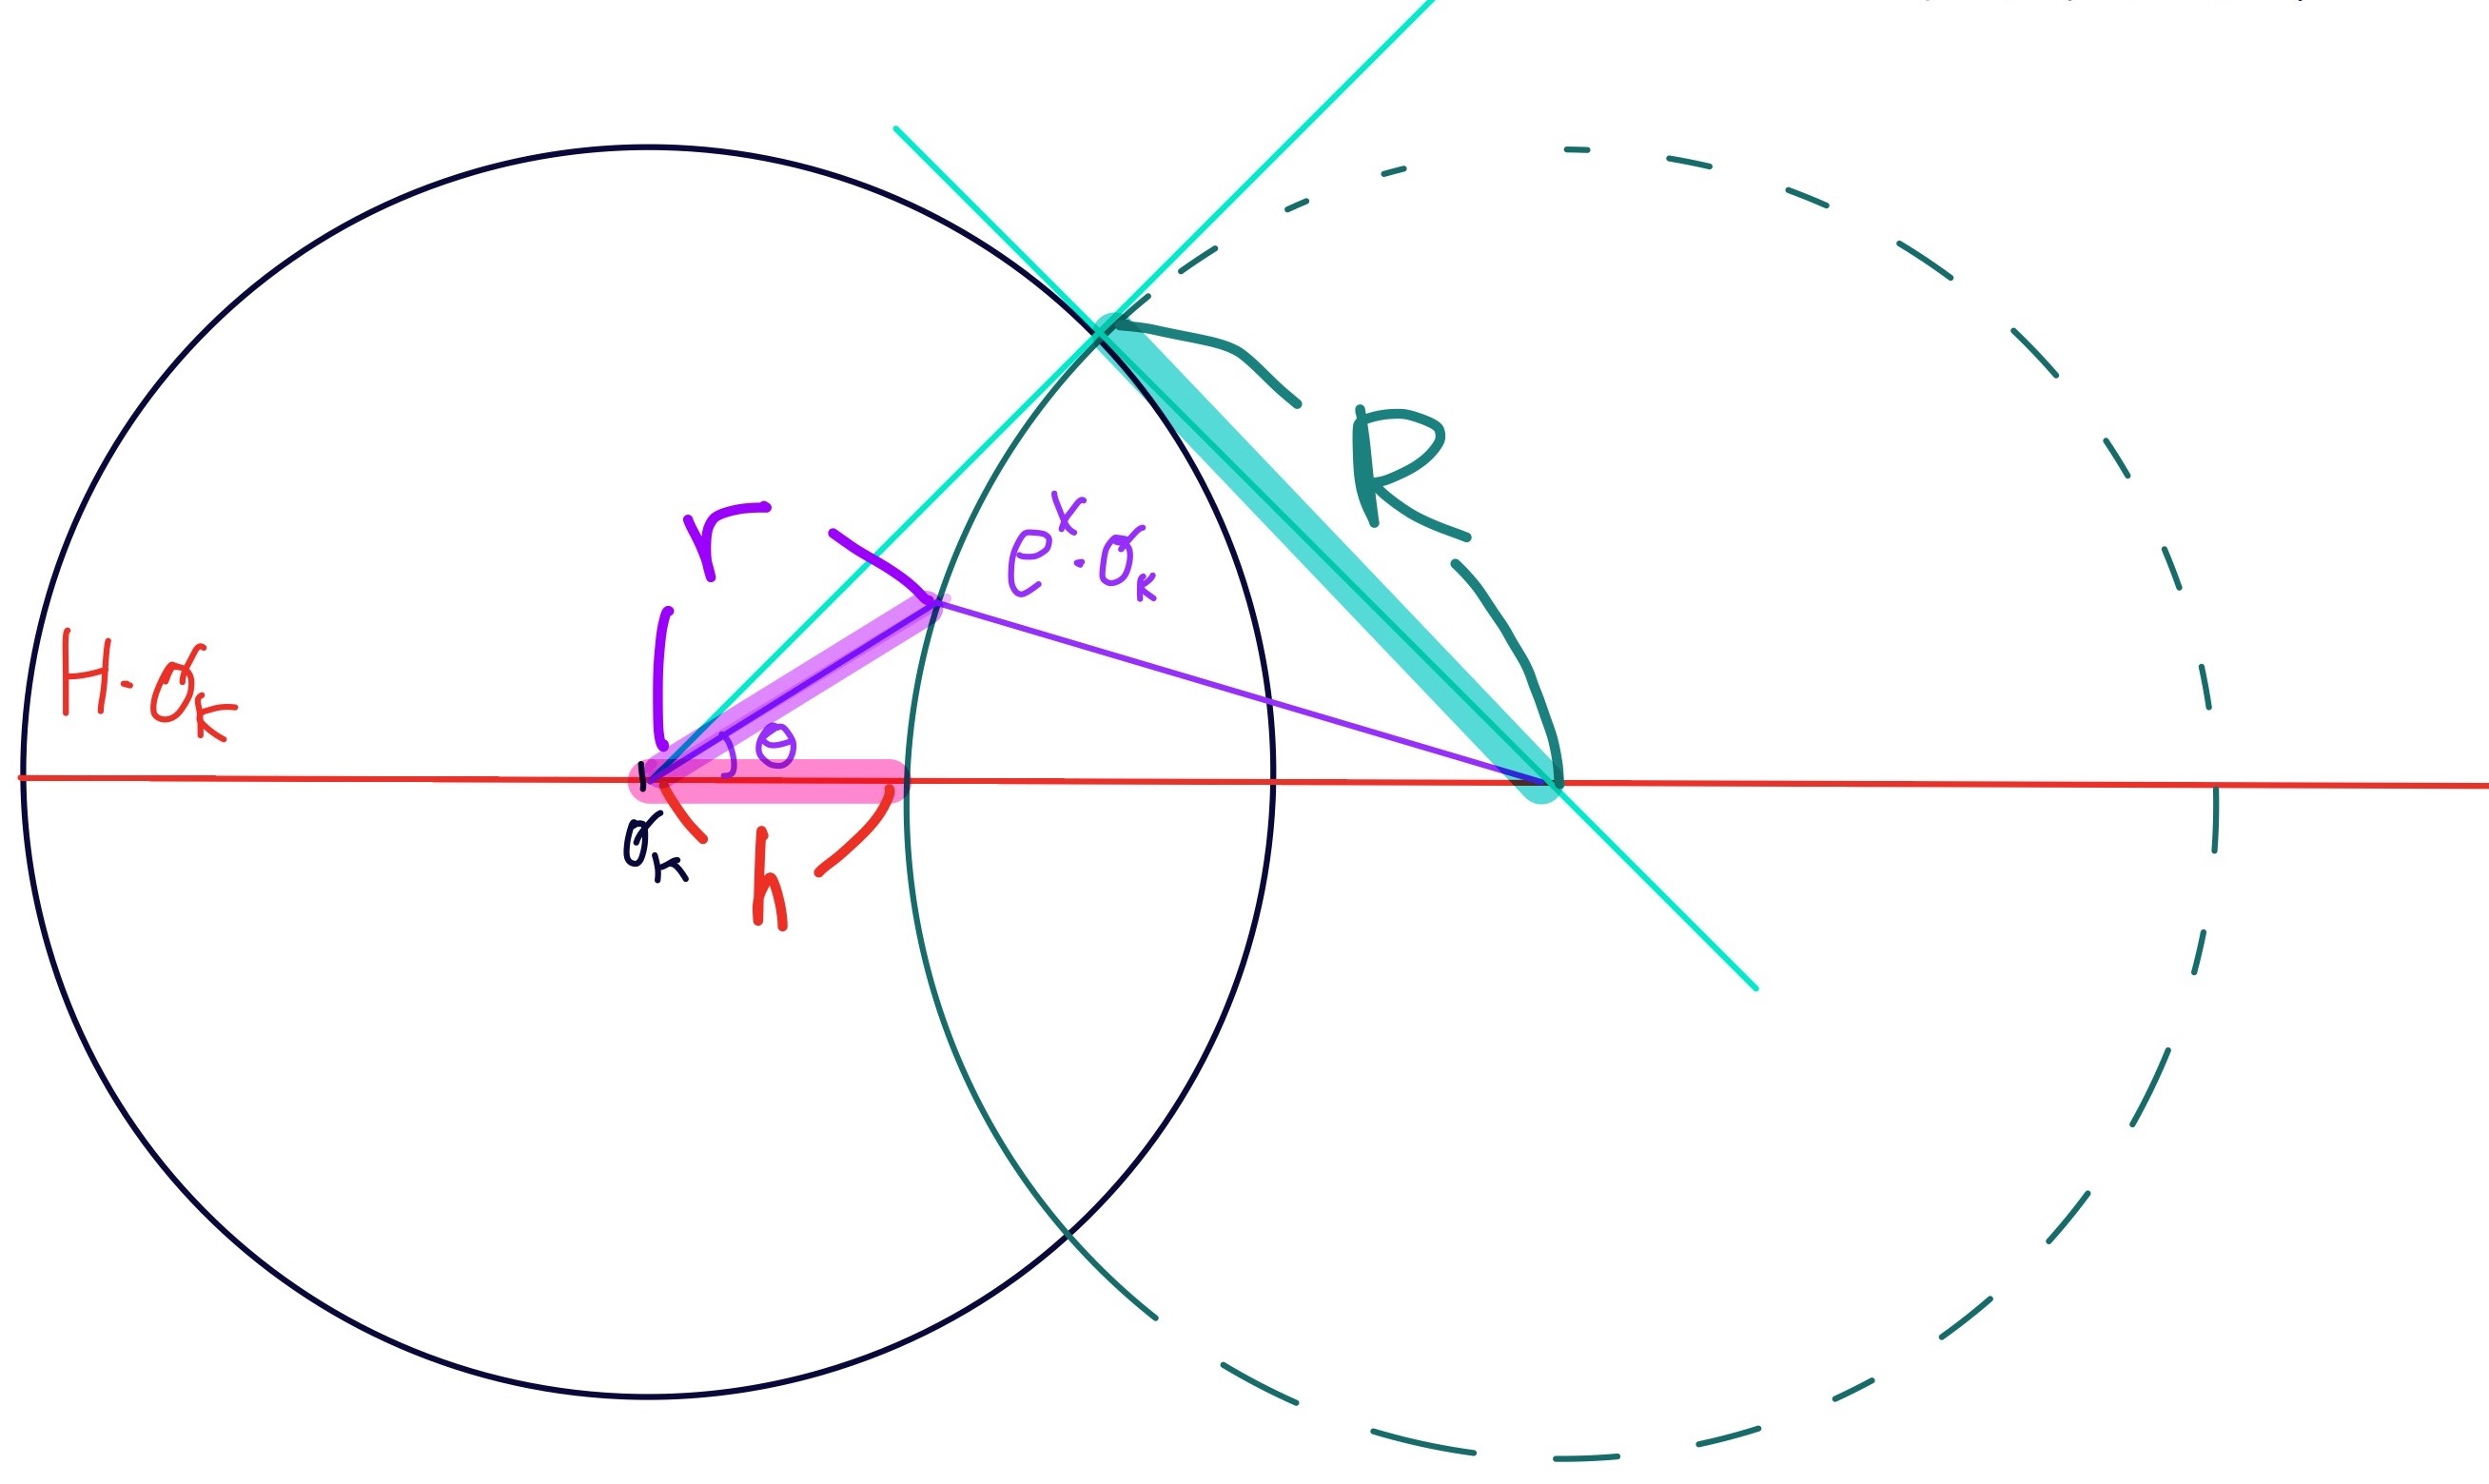
\includegraphics[scale=0.08]{../graph/prob-eg-1.jpg}
    % 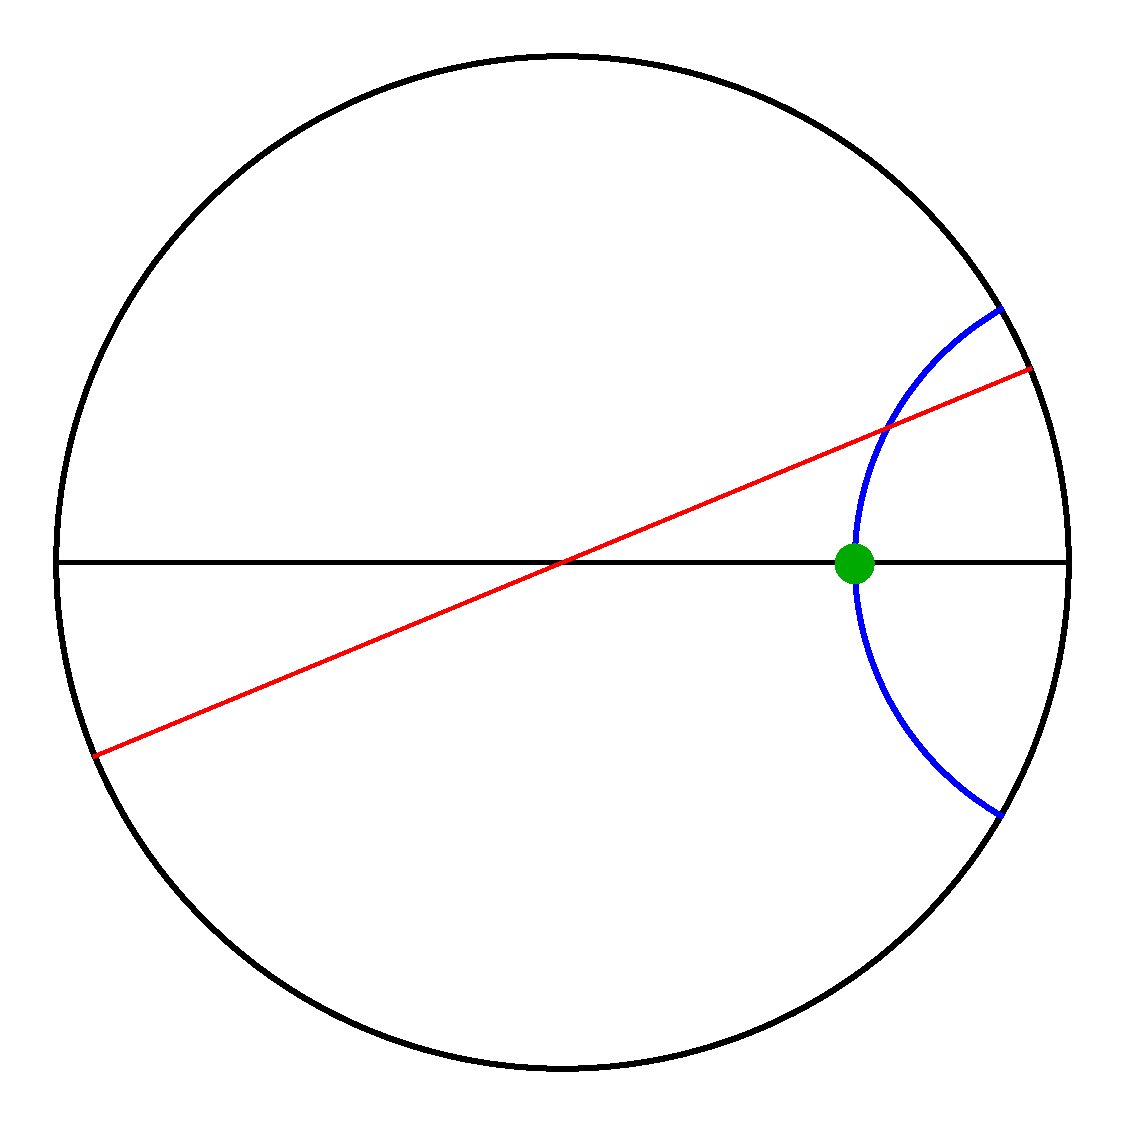
\includegraphics[scale=0.3]{../graph/y-and-z.pdf}
    \caption{}
    \label{fig:prob-eg-1}
  \end{figure}

  右の円の Euclid 距離での半径を$R$とし,$e^{tX_{\theta}}\cdot o_K $から$H\cdot o_K$への垂線の足の$o_K$からの Euclid 距離を$h$とするとき,外側の青色の直角三角形に対して三平方の定理を用いて$(h+R)^2 = R^2 +  1 $より$R = \dfrac{1-h^2}{2h}$,$R+h = \dfrac{1+h^2}{2h}  $を得る.

  さらに下の紫色の三角形に対して余弦定理を用いて${R^2 = (R+h)^2 + r^2 - 2r(R+h)\cos\theta }$を得,
  \begin{align*}
    R^2 &= (R+h)^2 + r^2 - 2(R+h) \cos\theta = R^2 +  1 + r^2 - 2r(R+h) \cos\theta                                   \\
                                            &= R^2 +  1 + r^2 - 2r\dfrac{1+h^2}{2h} \cos\theta  
  \end{align*}
  より
  \begin{align}
    {\dfrac{2r\cos\theta}{r^2 + 1} = \dfrac{2h}{h^2 + 1} }\label{eq:1018-main}
  \end{align}
  を得る.

  $r = \tanh t$,$h = \tanh s$であるから\Cref{eq:1018-main} は$\cos\theta \tanh 2t = \tanh 2t $と書き直せる.したがって$X_{\theta}$に対して$Y(\real X) $が有界であることと$ \abs{\cos\theta}\neq 1 \iff  X\nin \ha  $であることが同値である.
\end{npfwn}

\begin{rem}\label{rem:su11-by-angle}

  \Cref{prop:prob-eg}は角度を用いた議論によっても示すことができる.具体的には,計算により次の\Cref{lem:0106}が示せる.
  \begin{lem}\label{lem:0106}
    $e^{sY}e^{rZ}\cdot o_K =
    \begin{pmatrix}
      \cosh s & \sinh s\\ \sinh s & \cosh s
    \end{pmatrix}
    \sqrt{-1}\tanh r \in \SU(1,1)/\U(1) $,$s > 0$,$r\in \real$に対し,$\phi_{s,r}\defeq \measuredangle_{o_K}(e^{sY}e^{rZ}\cdot o_K, e^{sY}\cdot o_K) $は,$\tan \phi_{s,r} = \dfrac{\tanh 2r}{\sinh 2s} $を満たす.ただし$Y \defeq
  \begin{pmatrix}
    0 & 1\\ 1 & 0
  \end{pmatrix}
  $,$Z \defeq \begin{pmatrix}
    0 & \sqrt{-1} \\ -\sqrt{-1} & 0
  \end{pmatrix}$とする.
  \end{lem}  

  \Cref{lem:0106}により\Cref{prop:prob-eg}は次のように証明できる.
  任意の$0\neq s\in \real, r\in \real $に対し,
  \begin{align}
    \lim_{r\to -\infty}\tan \phi_{\abs{s},r} = \dfrac{-1}{\sinh 2\abs{s}}  \leq \tan \phi_{s,r} \leq  \lim_{r\to \infty}\tan \phi_{\abs{s},r} = \dfrac{1}{\sinh 2\abs{s}}\label{eq:0106}
  \end{align}
  であるから,$X\nin \real Y $の元に対して$Y(\real X) $が非有界であるとすると,$ 0 <  \epsilon < \phi(X,\ha)$なる$\epsilon$に対し,ある$t\in \real $が存在して,$Y(tX) = s_tY $,$\sinh 2\abs{s_t} > \dfrac{1}{\tan \epsilon} $である.$Z(tX) = r_tZ $とすると\Cref{eq:0106}より$\abs{\tan \phi_{s_t,r_t}} < \tan \epsilon $,したがって
  \begin{align*}
    -\epsilon < \measuredangle_{o_K}(e^{s_tY}e^{r_t Z}\cdot o_K, e^{s_tY}\cdot o_K) < \epsilon < \phi(X,\ha)
  \end{align*}
  となる.しかし定義より$\measuredangle_{o_K}(e^{s_tY}e^{r_t Z}\cdot o_K, e^{s_tY}\cdot o_K) = \measuredangle_{o_K}(e^{tX}\cdot o_K, e^{Y(tX) }\cdot o_K) $であり,$\measuredangle_{o_K}(e^{tX}\cdot o_K, e^{Y(tX) }\cdot o_K) = \phi(X,\ha\cap\pe)$であるから矛盾する. 

  
\end{rem}

\begin{cor}\label{cor:prob-eg}
  $G = \SO(1,n) $,$H = \SO(1,k) $,$1\leq k\leq n-1$に対して\Cref{prob:1121}は正しい.より具体的には次の\Cref{thm:1018-main}が成り立つ.
\end{cor}
\begin{thm}\label{thm:1018-main}
  % $\SO(n,1)/\SO(n) $を {\Poincare} ball model で実現したとき,
  $G = \SO(1,n) $,$H = \SO(1,k) $,$1\leq k\leq n-1$とする.
  $
  \begin{cases}
    \ds Y(X) &= \frac{1}{4}\inv{\tanh}[\tanh(4\norm{X})\cos\theta ]\frac{\pr(X)}{\norm{\pr(X)}},\quad X\in \pe\setminus (\per{\ha}\cap \pe) \\
    \ds Y(X)&= 0,\qquad \qquad\qquad\qquad\qquad\qquad\qquad\quad \ X\in  \per{(\ha)}\cap \pe
  \end{cases}
  $である.
\end{thm}
\begin{cor}
  $X\in \pe\setminus \ha $
  % $ e^{X}\cdot o_K\nin \SO(k,1)\cdot o_K $
  のとき,$0 \leq \cos \theta\neq 1$であり,\\
  $Y(\real X) = \lbig\{s\frac{\pr(X)}{\norm{\pr(X)}} \mid  -\frac{\inv{\tanh}(\cos\theta)}{4} < s < \frac{\inv{\tanh}(\cos\theta)}{4} \rbig\} $ (if $X\in \pe\setminus (\per{\ha}\cap \pe)$) \\
  あるいは$Y(\real X) = \{\bm{0}\}$ (if $X\in  \per{(\ha)}\cap \pe$) より,$\ha\cap \pe $内で有界である.
\end{cor}

\vspace{-1em}
\begin{defi}\textcolor{white}{hoge}

  \begin{easylist}[itemize]
    @ {\Poincare} ball の計量は$4\dfrac{\sum_i dx_i^2}{(1-x_i^2)^2} $とする.
    @ $\pr\colon \pe = (\ha\cap \pe)\oplus (\per{(\ha )}\cap \pe) \to (\ha\cap \pe)$を直交射影とする.
    @ $\cos \theta \defeq \frac{\lyama X, \pr(X)\ryama }{\norm{X}\, \norm{\pr(X)}} \geq 0 $,ただし$\lyama{-},{-}\ryama  $は$\solie(n,1) $の Killing form とする.
  \end{easylist}  
\end{defi}

\begin{lem}\label{lem:1018}
  $Z\in \pe$に対し,$e^Z \cdot o_K $が$o_K$から Euclid 距離で$\tanh p$,$p \geq 0$の位置にある場合,$\norm{Z} = \frac{p}{2} $である.
\end{lem}



\begin{npfwn}[{\Cref{cor:prob-eg}}]\bluetext{make it precise}
  $\SO(1,n)/\SO(n)$の開球としての実現を考える.「$e^X\cdot o_K $と$o_K$を結ぶ直線」と$H\cdot o_K$で張られる超平面で$\SO(1,n)/\SO(n)$を切った際の断面を考える.
  \begin{figure}[H]
    \centering
    % \raggedleft
    % \raggedrightp
    % \includegraphics[scale=0.08]{../graph/fig1.jpg}
    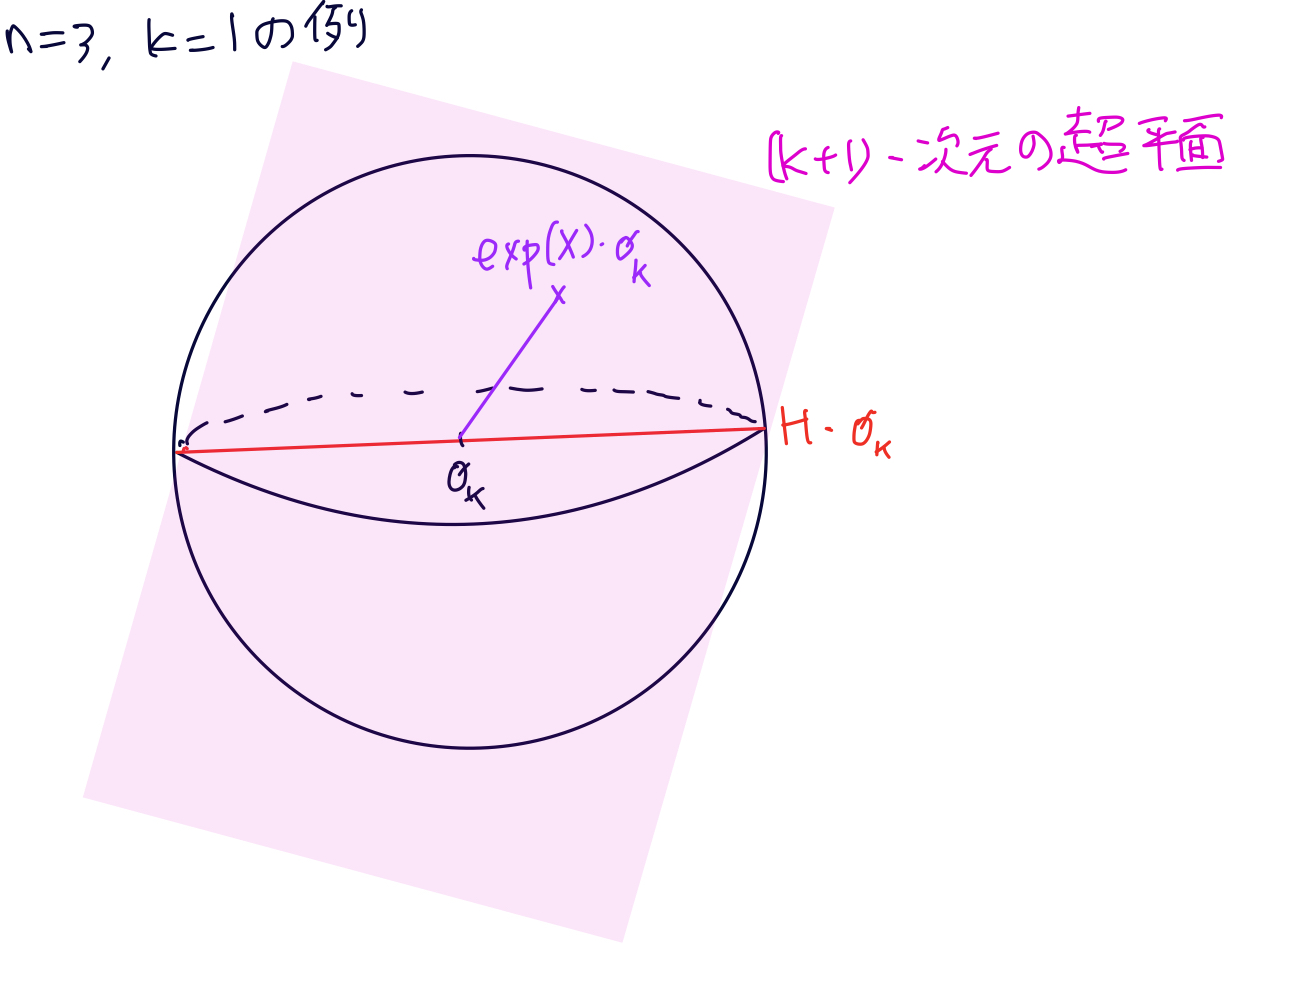
\includegraphics[scale=0.2]{../graph/son1-3.jpeg}
    \caption{}
    \label{fig:son1}
  \end{figure}
  
  この断面に現れるのは\Cref{fig:prob-eg-1}と同じであるから,同様の計算により\Cref{cor:prob-eg}を得る.

  よって\Cref{lem:1018}より,$\norm{Y(X)} = \frac{s}{2} = \frac{1}{4}\inv{\tanh}(\cos\theta \tanh 2t) $を得る.再び\Cref{lem:1018}より$4\norm{X} = 2t $であるから,$\norm{Y(X)} = \frac{1}{4}\inv{\tanh}[\tanh(4\norm{X})\cos\theta] $を得,\Cref{thm:1018-main}の主張が従う.  
\end{npfwn}


\subsection{\Cref{prob:1121} の観察: 類似の問いとその反例}

\Cref{prob:1121}は,$G$の実階数が1の場合は
\begin{prob}\label{prob:1121-2}

  $\pe_{H,\bdd} = \{X\in \pe\mid [X,(\ha\cap\pe)]\neq \{0\} \text{ あるいは } X\perp (\ha\cap\pe)\text{ である.}  \}  $となるか?
  
\end{prob}
と同値であった.しかし\Cref{prob:1121-2}には$G$の実階数が2の場合の反例が存在する.
\begin{prop}\label{prop:0114}
  $G = \SL(3,\real) $,$H = \{\diag(e^a,e^b,e^c)\mid a,b,c\in \real,\ a+ b + c = 0 \} $,$X\defeq
  \begin{pmatrix}
    1 & 0 & 0 \\
    0 & 0 & \sqrt{2} \\
    0 & \sqrt{2} & -1
  \end{pmatrix}
  $に対し$Y(\real X) $は非有界である.
\end{prop}


$\ha = \{\diag(a,b,c)\mid a,b,c\in \real,\ a +b + c = 0 \}  $であるから$X_1 = \diag(1,0,-1)$,$X_2 = \begin{pmatrix}
  0 & 0 & 0 \\
  0 & 0 & \sqrt{2} \\
  0 & \sqrt{2} & 0
\end{pmatrix}$であり,$[X_1, X_2] = \begin{pmatrix}
  0 & 0 & 0 \\
  0 & 0 & \sqrt{2} \\
  0 & -\sqrt{2} & 0
\end{pmatrix} \neq 0$より$X$は\Cref{eq:prob-1121}の右辺の集合の元ではあるが$X\nin \pe_{H,\bdd} $であるから,\Cref{prop:0114}は\Cref{prob:1121}の反例となっている.

1つ補題を用意してから\Cref{prop:0114}を証明する.
\begin{lem}\label{lem:0114}
  任意の$t\in \real$に対し
  \begin{align*}
    \exp\lbig(2t\begin{pmatrix}
      0 & \sqrt{2} \\
      \sqrt{2} & -1 
    \end{pmatrix}\rbig) &=
                 \begin{pmatrix}
                   \dfrac{2e^{2t} + e^{-4t}}{3} &  \dfrac{\sqrt{2} (e^{2t} - e^{-4t})}{3}\\
                   \\
                   \dfrac{\sqrt{2} (e^{2t} - e^{-4t})}{3} & \dfrac{e^{2t} + 2e^{-4t}}{3}
                 \end{pmatrix}
  \end{align*}
  である.
\end{lem}

\begin{npfwn}[\Cref{lem:0114}]

  $ \theta $を$\cos 2\theta = \dfrac{1}{3} $,$\sin 2\theta = \dfrac{-2\sqrt{2}}{3} $を満たす実数として任意に1つ固定する.このとき
  \begin{align*}
    \cos^2 \theta &= \dfrac{1 +\cos 2\theta}{2} = \dfrac{2}{3},\\
    \sin^2 \theta &= \dfrac{1-\cos 2\theta}{2} = \dfrac{1}{3}
  \end{align*}
  である.$k \defeq
  \begin{pmatrix}
    \cos \theta & -\sin \theta \\ \sin \theta & \cos \theta
  \end{pmatrix}
  $とすると,
  \begin{align*}
    k
    \begin{pmatrix}
      0 & \sqrt{2} \\
      \sqrt{2} & -1 
    \end{pmatrix}\inv{k} &=
                           \begin{pmatrix}
                             -2\sqrt{2}\sin\theta \cos\theta  - \sin^2\theta & \sqrt{2}(\cos^2 \theta - \sin^2\theta) + \cos\theta \sin\theta \\
                             \sqrt{2}(\cos^2 \theta - \sin^2\theta) + \cos\theta \sin\theta  & 2\sqrt{2}\sin\theta \cos\theta  - \cos^2\theta
                           \end{pmatrix}\\
        &=
          \begin{pmatrix}
            -\sqrt{2}\sin 2\theta  - \sin^2\theta & \sqrt{2}\cos 2\theta + \dfrac{\sin 2\theta}{2} \\
            \sqrt{2}\cos 2\theta + \dfrac{\sin 2\theta}{2}  &\sqrt{2}\sin 2 \theta - \cos^2\theta
          \end{pmatrix}\\
        &=
          \begin{pmatrix}
            1  &  0\\ 0 & -2
          \end{pmatrix}
  \end{align*}
  である.

  したがって
  \begin{align*}
    k\exp\lbig(2t\begin{pmatrix}
      0 & \sqrt{2} \\
      \sqrt{2} & -1 
    \end{pmatrix}\rbig)\inv{k} &= \exp
                                 \begin{pmatrix}
                                   2t & 0 \\ 0 & -4t
                                 \end{pmatrix}
  \end{align*}
  であるから,
  \begin{align*}
    \exp\lbig(2t\begin{pmatrix}
      0 & \sqrt{2} \\
      \sqrt{2} & -1 
    \end{pmatrix}\rbig) &= \inv{k} \exp\lbig(
                                 \begin{pmatrix}
                                   2t & 0 \\ 0 & -4t
                                 \end{pmatrix}\rbig)k\\
        &=
          \begin{pmatrix}
            \cos \theta  & \sin \theta \\ -\sin \theta & \cos \theta
          \end{pmatrix}
                                                         \begin{pmatrix}
                                                           e^{2t} & 0 \\ 0 & e^{-4t}
                                                         \end{pmatrix}
                                                                             \begin{pmatrix}
                                                                               \cos \theta  & -\sin \theta \\ \sin \theta & \cos \theta
                                                                             \end{pmatrix}\\
        &=
          \begin{pmatrix}
            e^{2t}\cos^2\theta + e^{-4t}\sin^2 \theta  & (e^{-4t} - e^{2t})\sin\theta \cos\theta \\ (e^{-4t} - e^{2t})\sin\theta \cos\theta  & e^{2t}\sin^2\theta +e^{-4t}\cos^2\theta
          \end{pmatrix}\\
        &= \begin{pmatrix}
          \dfrac{2e^{2t} + e^{-4t}}{3} &  \dfrac{\sqrt{2} (e^{2t} - e^{-4t})}{3}\\
          \\
          \dfrac{\sqrt{2} (e^{2t} - e^{-4t})}{3} & \dfrac{e^{2t} + 2e^{-4t}}{3}
                 \end{pmatrix}
  \end{align*}
\end{npfwn}

\begin{npfwn}[\Cref{prop:0114}]
  行列式1の$3\times 3$正定値実対称行列全体の集合$\Symm^{+}(3)$と$G/K$は$gK \mapsto g
  \begin{pmatrix}
    1 & 0\\ 0 & 1
  \end{pmatrix}
  \trans{g} $により微分同相である.
  
  \Cref{lem:0114}より
  \begin{align}
    e^{tX}\cdot o_K &= e^{tX}\; \trans{(e^{tX})} = e^{2tX}\notag\\
                    &= \begin{pmatrix}
                      e^{2t} & 0 & 0 \\
                      0 & \dfrac{2e^{2t} + e^{-4t}}{3} &  \dfrac{\sqrt{2} (e^{2t} - e^{-4t})}{3}\\
                      % \\
                      0 & \dfrac{\sqrt{2} (e^{2t} - e^{-4t})}{3} & \dfrac{e^{2t} + 2e^{-4t}}{3}
                    \end{pmatrix}\label{eq:0114-1}
  \end{align}
  である.

  $Y \defeq \diag(a,b,c)  $,$a + b + c = 0$,$Z \defeq
  \begin{pmatrix}
    0 & 0 & 0\\
    0 & 0 & 1\\
    0 & 1 & 0
  \end{pmatrix}
  $とすると,$r\in \real$に対し,
  \begin{align}
    e^{Y}e^{rZ}\cdot o_K &= e^{Y}e^{2rZ}e^{Y}\notag\\
                         &=
                           \begin{pmatrix}
                             e^{a} & 0 & 0 \\
                             0 & e^{b} & 0\\
                             0 & 0 & e^{c}
                           \end{pmatrix}
                                     \begin{pmatrix}
                                       1 & 0 & 0\\
                                       0 & \cosh 2r & \sinh 2r \\
                                       0 & \sinh 2r & \cosh 2r
                                     \end{pmatrix}
                                                      \begin{pmatrix}
                                                        e^{a} & 0 & 0 \\
                                                        0 & e^{b} & 0\\
                                                        0 & 0 & e^{c}
                                                      \end{pmatrix}\notag\\
                         &=
                           \begin{pmatrix}
                             e^{2a} & 0 & 0\\
                             0 & e^{2b}\cosh 2r & e^{b+c}\sinh 2r \\
                             0 & e^{b+c}\sinh 2r & e^{2c}\cosh 2r
                           \end{pmatrix}\notag\\
                         &= \begin{pmatrix}
                             e^{2a} & 0 & 0\\
                             0 & e^{2b}\cosh 2r & e^{-a}\sinh 2r \\
                             0 & e^{-a}\sinh 2r & e^{-2a-2b}\cosh 2r
                           \end{pmatrix}\label{eq:0114-2}
  \end{align}
  である.ただし最後の変形には$a + b + c = 0$を用いた.

  \Cref{eq:0114-1}と\Cref{eq:0114-2}を見比べると,
  \begin{align*}
    a &= t,\\
    \sinh 2r &= \dfrac{2\sqrt{2}}{3}\sinh 3t, \\
    e^{2b} &= \dfrac{2e^{2t} + e^{-4t}}{\sqrt{9 + 8\sinh^2 3t}}
  \end{align*}
  とすると$e^{Y}e^{rZ}\cdot o_K = e^{tX}\cdot o_K $を得る.つまり任意の$t\in \real$に対し
  \begin{itemize}
  \item $Y(tX) = \diag(a(t) ,b(t) ,-a(t) -b(t) ) $

    ただし$a(t) = t$,$b(t) =\dfrac{1}{2} \log \lbig(\dfrac{2e^{2t} + e^{-4t}}{\sqrt{9 + 8\sinh^2 3t}}\rbig) $,
  \item $Z(tX) = r(t)Z  $ただし$r(t) = \dfrac{1}{2} \inv{\sinh}\lbig( \dfrac{2\sqrt{2}}{3}\sinh 3t\rbig) $
  \end{itemize}
  であるから,$Y(\real X) $は非有界である.  
\end{npfwn}



$G$が実階数1の場合に限っても\Cref{prob:1121-2}と類似の問題はいくつか考えられる.例えば$\ha\cap\pe$を$\ha$に置き換えた次の問題が立てられる.
\begin{prob}\label{prob:1101}
  $\pe_{H,\bdd} = \{X\in \pe\mid  [X,\ha]\neq \{0\} \text{ あるいは } X\perp \ha \text{ である.}\}  $となるか?
\end{prob}

しかし\Cref{prob:1101}にも反例が存在する.
\begin{lem}\label{lem:1118-main}
  $G = \SL(3,\real) $,$Y_1\defeq \diag(1,1,-2)$,$Y_2 \defeq \begin{pmatrix}
    0 & 1 & 0\\
    -1 & 0 & 0 \\
    0 & 0 & 0
  \end{pmatrix}$,\\
  $\ha = \real Y_1 \oplus \real Y_2 $,$X = \diag(1,0,-1) $に対し,$[X,\ha] \neq \{0\} $であるが$Y(\real X) = \real Y_1 $であり,非有界である.
\end{lem}

\begin{ncalcof}[\Cref{lem:1118-main}]

  $\ha$は可換Lie環であり,$\ge = \slie(3,\real) $のCartan対合$\theta W \defeq -\trans{W} $に対し$\ha = \theta \ha$である.

  $[X,\ha]\neq 0 $は,$[X, Y_2] \neq 0$より従う.

  ここで$Z_1\defeq \diag(1,-1,0)\in \per{\ha}\cap \pe $であり,任意の$t\in \real$に対し,$e^{2tX} = e^{tY_1}e^{tZ_1} $であるから,$Y(\real X) = \real Y_1 $となり,\Cref{lem:1118-main} が示された.
\end{ncalcof}

\Cref{lem:1118-main}において$X$と$\ha$は,$[X,\ha] \neq \{0\} $だが$[X,(\ha\cap \pe)] = \{0\}$かつ$X\not\perp (\ha\cap \pe) $となるように取った.したがって\Cref{prob:1101}の右辺を次の\Cref{prob:1101-2}のように少し弱めても\Cref{lem:1118-main}はその反例になっている.
\begin{prob}\label{prob:1101-2}
  $\pe_{H,\bdd} = \{X\in \pe\mid  [X,\ha]\neq \{0\} \text{ あるいは } X\perp (\ha\cap\pe) \text{ である.} \}  $となるか?
\end{prob}



\section{具体例と主定理の証明}
\subsection{具体例: 実階数1の古典型単純Lie群}
\begin{prop}\label{prop:classical-rank-one}
  $G = \SO(1,n)$,$ \SU(1, n)$,$\Sp(1,n) $,$H = \SO(1,1) $,$n\geq 2$に対して\Cref{prob:1121} は正しい.
\end{prop}

$G = \Sp(1,2) $,$\ha = \real \begin{pmatrix}
    0 & 1 & 0 \\
    1 & 0 & 0\\
    0 & 0 & 0
  \end{pmatrix}$の場合にのみ示す.その他の場合も全く同様の議論である.
\begin{prop}\label{prop:1127-main}
  $G = \Sp(1,2) $,$H = \SO(1,1)$,$X\in \pe$に対し,$Y(\real X) $が有界であることと$ X\in \{0\}\cup \pe\setminus \ha  $であることは同値である.
\end{prop}

ただし,$H$は$G$の左上に入っている.すなわち,$\Lie H = \ha = \real Y $,$Y\defeq \begin{pmatrix}
  0 & 1 & 0 \\
  1 & 0 & 0\\
  0 & 0 & 0
\end{pmatrix}$とする.

\begin{nttdef}
  
  $\quat$を四元数体とする.${\Sp(1,2)\defeq \{g\in \GL(3,\quat)\mid \bar{\trans{g}}\; I_{1,2}g = I_{1,2}  \}} $,$I_{1,2} \defeq \diag(-1,1,1) $とし,$\Sp(1,2) $の$\quat^3 $への自然表現を,$
  \begin{pmatrix}
    x_{11} & x_{12} & x_{13}\\ x_{21} & x_{22} & x_{23}\\ x_{31} & x_{32} & x_{33}
  \end{pmatrix}\cdot
  \begin{pmatrix}
    a \\ b \\c
  \end{pmatrix}
  =
  \begin{pmatrix}
    x_{11}a + x_{12}b + x_{13}c\\ x_{21}a + x_{22}b + x_{23}c\\ x_{31}a + x_{32}b + x_{33}c\\    
  \end{pmatrix}
  $により定める.
  
  $\Sp(1,2)/\Sp(1)\times \Sp(2) \simeq \{(z_1, z_2)\mid z_1,z_2\in \quat ,\; \abs{z_1}^2 + \abs{z_2}^2   < 1 \} =: \quat\mathbb{H}^2 $である.なぜならば$\trans{(1,0,0)} $の自然表現$\Sp(1,2)\leftaction \quat^2 $による軌道を考え,第2,第3成分に第1成分の逆数を右からかけた空間が$\quat\mathbb{H}^2$と微分同相であるためであり,$\Sp(1,2)\leftaction \trans{(1,0,0)} $による軌道上の点$
  \begin{pmatrix}
    z_0 \\ z_1 \\ z_2 
  \end{pmatrix}
  $に対応する$\quat\mathbb{H}^2$の点を$
  \lbig[ \begin{pmatrix}
    z_0 \\ z_1 \\ z_2 
  \end{pmatrix}\rbig] = \lbig[ \begin{pmatrix}
    1 \\ z_1\inv{z_0} \\ z_2\inv{z_0} 
  \end{pmatrix}\rbig] 
  $と書く.
\end{nttdef}

行列計算により,次が示される.
\begin{lem}\label{lem:exp-quat}
  
  $\forall z,w\in \quat$に対し,$\exp
  \begin{pmatrix}
    0 & z & w  \\
    \bar{z} & 0 & 0\\
    \bar{w} & 0 & 0
  \end{pmatrix}
  =
  \begin{pmatrix}
    \cosh r &  \ast & \ast \\
    \\
    \dfrac{\bar{z}}{r} \sinh r &  \ast & \ast \\
    \\
    \dfrac{\bar{w}}{r}\sinh r &  \ast & \ast 
  \end{pmatrix}
  $,ただし$r \defeq \sqrt{\abs{z}^2 + \abs{w}^2 } $,である.
\end{lem}

\begin{npfwn}[\Cref{prop:1127-main}]
  
  % $\Lie H = \ha = \real A $,$A\defeq \begin{pmatrix}
  %   0 & 1 & 0 \\
  %   1 & 0 & 0\\
  %   0 & 0 & 0
  % \end{pmatrix}$とする.
  $X = 0$ならば$ Y(\real X) = \{0\} $と$X\in \ha\setminus\{0\} $のときに$Y(\real X) $が非有界であることは明らかであるから,$X\nin \ha $の場合にのみ議論すればよい.% つまり
  % $X =
  % \begin{pmatrix}
  %   0 & z & w \\
  %   \bar{z} & 0 & 0 \\
  %   \bar{w} & 0 & 0 
  % \end{pmatrix}
  % \in \pe\setminus\ha $,$z,w\in \quat \st \abs{z}^2 +\abs{w}^2  = 1 $を任意に1つ固定して議論して一般性を失わない.このとき,$X\in\pe\setminus \ha $より$\re z \neq \pm 1$であることに注意する ($\re\colon \quat\ni a+bi+cj+dk\mapsto a\in \real$とする).

  $G$の Cartan 対合を$\Theta(g) = \inv{(g^{*})} $ ($g^{*}$は$g$の共役転置) とするとき,$\Theta(e^{Y(tX)}e^{Z(tX)})\cdot o_K = e^{-Y(tX)}e^{-Z(tX)}\cdot o_K = \Theta(e^{X})\cdot o_K = e^{-X}\cdot o_K $より,$Y(\real X) $が非有界であることと$ Y(\real X)\subset \real Y $が上に非有界であることは同値である.

  したがって,$Y (\real X) $が非有界であるとき,列$\{t_n \in \real \}_{n\in \nat} $で,$s_n\to \infty,\; n\to \infty$,ただし$Y(t_n X) = s_n Y$,なるものが存在する.

  また,任意の$\per{\ha}\cap\pe $の元はある$Z =
  \begin{pmatrix}
    0 & z & w \\
    \bar{z} & 0 & 0 \\
    \bar{w} & 0 & 0 
  \end{pmatrix} \in \per{\ha}\cap\pe $,$z,w\in \quat \st \abs{z}^2 +\abs{w}^2  = 1 $と$r\in \real$により$rZ$と表せる.$Z(t_nX) = r_nZ_n$,$Z_n\defeq \begin{pmatrix}
    0 & z_n & w_n \\
    \bar{z_n} & 0 & 0 \\
    \bar{w_n} & 0 & 0 
  \end{pmatrix} $,$z_n,w_n\in \quat \st \abs{z_n}^2 +\abs{w_n}^2  = 1 $とすると,$X\nin\ha$であるから\Cref{thm:kob97}より$\abs{r_n}\to \infty $である.$z_n,w_n\in \quat \st \abs{z_n}^2 +\abs{w_n}^2  = 1 $より,$\{t_n\} $の部分列を取るとある$Z_{\infty} $が存在して$\lim_{n\to \infty}Z_n = Z_{\infty} =
  \begin{pmatrix}
    0 & z_{\infty} & w_{\infty} \\
    \bar{z_{\infty}} & 0 & 0 \\
    \bar{w_{\infty}} & 0 & 0 
  \end{pmatrix}
  \in \per{\ha}\cap\pe $なるようにできる.$Z\in\pe\setminus \ha $より$\re z_{\infty} \neq \pm 1$であることに注意する ($\re\colon \quat\ni a+bi+cj+dk\mapsto a\in \real$とする).

  \Cref{lem:exp-quat}より, 
  \begin{align*}
    e^{s_n Y}e^{r_n Z_n}\cdot o_K &=
    \begin{pmatrix}
      \cosh s_n & \sinh s_n & 0 \\
      \sinh s_n & \cosh s_n & 0 \\
      0 & 0 & 1 
    \end{pmatrix}
              \lbig[\begin{pmatrix}
                1\\ \pm \bar{z_n} \tanh \abs{r_n}  \\ \pm \bar{w_n} \tanh \abs{r_n}
              \end{pmatrix}\rbig]\\
    &=  \lbig[ \begin{pmatrix}
      \cosh s_n \pm \bar{z_n} \tanh \abs{r_n} \sinh s_n \\ \sinh s_n \pm \bar{z_n} \tanh \abs{r_n} \cosh s_n \\ \pm \bar{w_n} \tanh \abs{r_n}
    \end{pmatrix}\rbig],
  \end{align*}
  複号は$r_n$の符号$\pm$と同順,である.このとき$\lim_{n\to \infty}\tanh s_n = 1 = \lim_{n\to \infty}\tanh \abs{r_n} $と$\lim_{n\to \infty} \re z_n = \re z_{\infty} \neq \pm 1$に注意すると次を得る.具体的な計算は後述する.
  \begin{align}
    \lim_{n\to \infty}(\sinh s_n \pm \bar{z_n} \tanh \abs{r_n} \cosh s_n)\inv{(\cosh s_n \pm \bar{z_n} \tanh \abs{r_n} \sinh s_n) } = 1\label{eq:-1}
  \end{align}
  である.

  したがって,$
  \begin{pmatrix}
    0 \\ 0 
  \end{pmatrix}
  \in \quat\mathbb{H}^2 $から$
  \begin{pmatrix}
    1 \\ 0 
  \end{pmatrix}
  \in \quat\mathbb{H}^2 $へのベクトルと,$
  \begin{pmatrix}
    0 \\ 0 
  \end{pmatrix}
  \in \quat\mathbb{H}^2 $から\\
  $ \begin{pmatrix}
    (\sinh s_n \pm \bar{z_n} \tanh \abs{r_n} \cosh s_n)\inv{(\cosh s_n \pm \bar{z_n} \tanh \abs{r_n} \sinh s_n) } \\  \ast 
  \end{pmatrix}\in \quat\mathbb{H}^2 $へのベクトルがなすEuclideanな内積の値を $I_n$とすると,$\lim_{n\to \infty}I_n = 1 $である.

  しかし,$
  \begin{pmatrix}
    0 \\ 0 
  \end{pmatrix}
  \in \quat\mathbb{H}^2 $から$
  \begin{pmatrix}
    1 \\ 0
  \end{pmatrix}
  \in \quat\mathbb{H}^2 $へのベクトルと,$
  \begin{pmatrix}
    0 \\ 0 
  \end{pmatrix}
  \in \quat\mathbb{H}^2 $から$e^{t_nX}\cdot o_K \in \quat \mathbb{H}^2 $へのベクトルがなすEuclideanな内積の値$J_n$は,$X \defeq   \begin{pmatrix}
    0 & z_0 & w_0 \\
    \bar{z_0} & 0 & 0 \\
    \bar{w_0} & 0 & 0 
  \end{pmatrix}$,$z_0,w_0\in \quat \st \abs{z_0}^2 +\abs{w_0}^2  = 1 $とするとき$J_n = \dfrac{\bar{z_0}}{r_0}\tanh (tr_0) $,$r_0\defeq \sqrt{\abs{z_0}^2 + \abs{w_0}^2 } $であり,$X\nin \ha \iff z_0\neq 1$より$\lim_{n\to \infty}J_n = \dfrac{\bar{z_0}}{r_0}\neq 1 $である.

  $e^{s_n Y}e^{r_n Z_n}\cdot o_K = e^{t_n X}\cdot o_K$より$ \lim_{n\to \infty} I_n = \lim_{n\to \infty}J_n  $であるが,以上2つの議論を合わせると$\lim_{n\to \infty} I_n= 1$,$\lim_{n\to \infty}J_n \neq 1 $であるから矛盾する.
  

  以上より「$X\in \pe\setminus\ha$ならば$Y(\real X) $有界」,したがって \Cref{prop:1127-main} を得る.  
\end{npfwn}


\begin{ncalcof}[\Cref{prop:1127-main}]
    
  \begin{align*}
    \lim_{n\to \infty}\abs{(\sinh s_n \pm \bar{z_n} \tanh \abs{r_n} \cosh s_n)\inv{(\cosh s_n \pm \bar{z_n} \tanh \abs{r_n} \sinh s_n) } - 1} = 0
  \end{align*}
  を示せば主張が得られる.具体的に計算すると,
  \begin{align}
    &\lim_{n\to \infty}\abs{(\sinh s_n \pm \bar{z_n} \tanh \abs{r_n} \cosh s_n)\inv{(\cosh s_n \pm \bar{z_n} \tanh \abs{r_n} \sinh s_n) } - 1}\notag \\
    % &\qquad\qquad\qquad \text{($\text{(この極限)} = 0$を示せば良い)} \\
    = & \lim_{n\to \infty}\lbig|\frac{(\tanh s_n\pm \bar{z_n}\tanh \abs{r_n})(1 \pm z_n \tanh\abs{r_n}\tanh s_n )}{\abs{(1 \pm \bar{z_n} \tanh\abs{r_n}\tanh s_n )}^2} - 1 \rbig|\notag \\    
    = & \lim_{n\to \infty}\frac{\abs{(\tanh s_n\pm \bar{z_n}\tanh \abs{r_n})z_n' - (1 \pm \bar{z_n} \tanh\abs{r_n}\tanh s_n )z_n' }}{\abs{(1 \pm \bar{z_n} \tanh\abs{r_n}\tanh s_n )}^2}\label{eq:ast} \tag{$\ast$}
  \end{align}
  である.ここで$ z_n'\defeq 1 \pm z_n\tanh\abs{r_n}\tanh s_n$とすると,
  \begin{align*}
    (\ast) &= \lim_{n\to \infty}\frac{\abs{(\tanh s_n\pm \bar{z_n}\tanh \abs{r_n})z_n' - (1 \pm \bar{z_n} \tanh\abs{r_n}\tanh s_n )z_n' }}{\abs{(1 \pm \bar{z_n} \tanh\abs{r_n}\tanh s_n )}^2}\\
    = & \lim_{n\to \infty}\frac{\abs{(1-\tanh s_n)(-1\pm \bar{z_n}\tanh \abs{r_n} )z_n'}}{\abs{(1 \pm \bar{z_n} \tanh\abs{r_n}\tanh s_n )}^2} \\
    = & \lim_{n\to \infty}\frac{\abs{(1-\tanh s_n)(-1\pm \bar{z_n}\tanh \abs{r_n} )}}{\abs{(1 \pm \bar{z_n} \tanh\abs{r_n}\tanh s_n )}} 
  \end{align*}
  であり,
  $0 < \min{\abs{1\pm \re z_n}}\leq  \abs{(1 \pm \bar{z_n} \tanh\abs{r_n}\tanh s_n )}\leq \sqrt{2^2 + 1^2} = \sqrt{5} $と$\min\{\abs{-1\pm \re z_n } \}  \leq \abs{-1\pm\bar{z_n}\tanh \abs{r_n} } \leq \sqrt{5} $であることと$\lim_{n\to \infty} \re z_n = \re z_{\infty} \neq \pm 1$より,
    \begin{align*}
      0 = \lim_{n\to \infty}(1-\tanh s_n)\frac{\min\{\abs{-1\pm \re z_n} \}}{\sqrt{5}}  &\leq \lim_{n\to \infty}\frac{\abs{(1-\tanh s_n)(-1\pm \bar{z_n}\tanh \abs{r_n} )}}{\abs{(1 \pm \bar{z_n} \tanh\abs{r_n}\tanh s_n )}}\\
      &\leq \lim_{n\to \infty}(1-\tanh s_n)\frac{\sqrt{5}}{\min\{\abs{1\pm \re z_n} \}} = 0
    \end{align*}
    を得,\Cref{eq:-1} が成り立つ.
\end{ncalcof}


%%% Local Variables:
%%% mode: latex
%%% TeX-master: "okuda-master-thesis"
%%% End:

\subsection{$ G$の実階数が1の場合}

\begin{thm}\label{thm:1216-main}
  $G$を実階数1の実半単純Lie群,$H$を$G$の非コンパクトな閉部分Lie群で,$G$のCartan対合$\Theta$に対して$\Theta H = H$かつ$\dim \ha\cap\pe = 1$とするとき,\Cref{prob:1121}が成り立つ.
\end{thm}

\begin{thm}\label{thm:0810}(\cite[p.~409, Theorem~3.1]{hel01},$\SU(2,1) $-reduction)
  $\ge = \ka \oplus \pe$を実半単純Lie環$\ge$のCartan対合$\theta$に対する Cartan分解とし,$\alpha,2\alpha\in \Sigma(\ge,\ah) $と仮定する.$0\neq X_{\alpha}\in \ge_{\alpha} $,$0\neq X_{2\alpha}\in \ge_{2\alpha} $を任意に固定したとき,$X_{\alpha},X_{2\alpha}, \theta X_{\alpha}, \theta X_{2\alpha} $から生成されるLie環$\ge^{*} $は$\sulie(2,1)$と同型である.
  
\end{thm}
以下で\Cref{thm:0810}を示すための補題や記号を設定し,\Cref{thm:0810}を示す.
\begin{nttdef}\label{nttdef:su21-red}
  \leavevmode
  \vspace{-1em}
  \begin{itemize}
  \item $\ah \subset \ge$を極大分裂可換部分代数,$\emm \defeq \zet_{\ka}(\ah) \defeq \{W\in \ka\mid [W,\ah] = \{0\} \} $とする.$B$を$\ge$のKilling 形式とする.
  \item $\Sigma(\ge,\ah) $を$\ah$に関する制限ルート系とする.$\ge_{\lambda} $を$\lambda\in \ah^{*}$のルート空間とする.
  \item $Y_{\alpha}\defeq [\theta X_{\alpha}, X_{2\alpha}] $とする.
  \item $A_{\alpha}\in \ah $を,任意の$H\in \ah$に対して$B(H,A_{\alpha}) = \alpha(H) $を満たす元とする.
    
    このとき,任意の$H\in \ah$に対して$B(H, [X_{\alpha}, \theta X_{\alpha}]) = \alpha(H) B(X_{\alpha}, \theta X_{\alpha}) $である.したがって
      \begin{align*}
        [X_{\alpha}, \theta X_{\alpha}] &= B(X_{\alpha}, \theta X_{\alpha})A_{\alpha} ,\\
        [Y_{\alpha}, \theta Y_{\alpha}] &= B(Y_{\alpha}, \theta Y_{\alpha})A_{\alpha}, \\
        [X_{2\alpha}, \theta X_{2\alpha}] &= 2B(X_{2\alpha}, \theta X_{2\alpha})A_{\alpha} 
      \end{align*}
    である.
    \item $c_{\alpha}\defeq \sqrt{\dfrac{-2}{\alpha(A_{\alpha})B(X_{\alpha}, \theta X_{\alpha})}} $,$ c_{2\alpha}  \defeq \sqrt{\dfrac{-2}{\alpha(A_{\alpha})B(X_{2\alpha}, \theta X_{2\alpha})}} $とし,
      \begin{align*}
        X_{\alpha}^{*} &\defeq c_{\alpha}X_{\alpha}, \\
        X_{2\alpha}^{*} &\defeq c_{2\alpha}X_{2\alpha},\\ 
        Y_{\alpha}^{*} &\defeq [\theta X_{\alpha}^{*}, X_{2\alpha}^{*} ] = c_{\alpha}c_{2\alpha}Y_{\alpha} ,\\
        A_{\alpha}^{*} &\defeq \dfrac{1}{12\alpha(A_{\alpha}) % \lyama \alpha, \alpha\ryama
      }A_{\alpha} 
      \end{align*}
    とする.
  \end{itemize}
\end{nttdef}

\begin{lem}\label{lem:3.2}
  $c \defeq 2\alpha(A_{\alpha})B(X_{\alpha},\theta X_{\alpha}) $とすると,$[X_{\alpha}, Y_{\alpha}] = cX_{2\alpha} $である.特に$0\neq Y_{\alpha}\neq X_{\alpha} $である.
\end{lem}
\begin{npfwn}[\Cref{lem:3.2}]
  Jacobi恒等式より
  \begin{align*}
    [X_{\alpha},[\theta X_{\alpha}, X_{2\alpha}]] + [\theta X_{\alpha},[X_{2\alpha}, X_{\alpha}]] + [X_{2\alpha},[X_{\alpha}, \theta X_{\alpha}]] = 0
  \end{align*}
  であり,$3\alpha\nin \Sigma(\ge,\ah) $より第二項が0となることから従う.
\end{npfwn}

\begin{lem}\label{lem:3.3}
  $[X_{\alpha},\theta Y_{\alpha}]\in \emm\setminus\{0\} $である.また$[[X_{\alpha}, \theta Y_{\alpha}], X_{\alpha}] = -3\alpha(A_{\alpha})B(X_{\alpha}, \theta X_{\alpha})Y_{\alpha} $である.
\end{lem}

\begin{npfwn}[\Cref{lem:3.3}]
  $Y_{\alpha} \in \ge_{\alpha} $より$[X_{\alpha},\theta Y_{\alpha}]\in \emm+ \ah$であり,任意の$H\in \ah$に対して
  \begin{align*}
    B(H, [X_{\alpha},\theta Y_{\alpha}]) &= B([H, X_{\alpha}], Y_{\alpha}) = \alpha(H) B(X_{\alpha}, [X_{\alpha}, \theta X_{2\alpha}]) \\
                                         &= \alpha(H)B([X_{\alpha}, X_{\alpha}], X_{2\alpha}) \\
                                         &= 0
  \end{align*}
  であることより$[X_{\alpha},\theta Y_{\alpha}]\in \emm$である.

  さらに,
  \begin{align*}
    [[\theta X_{\alpha},Y_{\alpha}], X_{\alpha}] &= -[[Y_{\alpha}, X_{\alpha}], \theta X_{\alpha}] - [[X_{\alpha}, \theta X_{\alpha}], Y_{\alpha}]\\
                                                 &= c[X_{2\alpha}, \theta X_{\alpha}] -  B(X_{\alpha},\theta X_{\alpha})\alpha(A_{\alpha})Y_{\alpha}\\
                                                 &= -cY_{\alpha}-  B(X_{\alpha},\theta X_{\alpha})\alpha(A_{\alpha})Y_{\alpha} \\
                                                 &= -3\alpha(A_{\alpha})B(X_{\alpha}, \theta X_{\alpha})Y_{\alpha} \neq 0
  \end{align*}
  より,$\theta [\theta X_{\alpha},Y_{\alpha}] = [X_{\alpha},\theta Y_{\alpha}]\in \emm\setminus\{0\} $である.
\end{npfwn}

\vspace{-1em}
\begin{lem}\label{lem:3.4}  
  $\real X_{\alpha} + \real Y_{\alpha} $は$\ad_{\ge}([X_{\alpha}, \theta Y_{\alpha}]) $で不変である.  
  さらに
  \begin{align*}
    [[X_{\alpha}, \theta Y_{\alpha}], Y_{\alpha}] &= -6\alpha(A_{\alpha})^2B(X_{\alpha}, \theta X_{\alpha})B(X_{2\alpha}, \theta X_{2\alpha})X_{\alpha},\\
  [Y_{\alpha}, \theta Y_{\alpha}] &= -2\alpha(A_{\alpha})B(X_{\alpha}, \theta X_{\alpha})B(X_{2\alpha}, \theta X_{2\alpha})A_{\alpha}
  \end{align*}
  である.

\end{lem}

\begin{npfwn}[\Cref{lem:3.4}]
  $[[X_{\alpha}, \theta Y_{\alpha}], Y_{\alpha}]  \in \real X_{\alpha} $を示せば,\Cref{lem:3.3} と併せて \Cref{lem:3.4} が従う.

  
  \begin{align*}
    [[X_{\alpha}, \theta Y_{\alpha}], Y_{\alpha}] &= -[[\theta Y_{\alpha}, Y_{\alpha}], X_{\alpha}] - [[Y_{\alpha}, X_{\alpha}], \theta Y_{\alpha}] \\
                                                  &= B(Y_{\alpha}, \theta Y_{\alpha})\alpha(A_{\alpha})X_{\alpha} +c[X_{2\alpha},[X_{\alpha}, \theta X_{2\alpha}]] \\
                                                  &= B(Y_{\alpha}, \theta Y_{\alpha})\alpha(A_{\alpha})X_{\alpha} - c[X_{\alpha}, [\theta X_{2\alpha}, X_{2\alpha}]] - c[\theta X_{2\alpha},[X_{2\alpha},X_{\alpha}]] \\
                                                  &= B(Y_{\alpha}, \theta Y_{\alpha})\alpha(A_{\alpha})X_{\alpha} - cB(X_{2\alpha},\theta X_{2\alpha})\alpha(A_{2\alpha})X_{\alpha}
  \end{align*}
  であり ($ \ge_{3\alpha} = \{0\} $による),$A_{2\alpha} = 2A_{\alpha} $であるから,
  \begin{align*}
[[X_{\alpha}, \theta Y_{\alpha}], Y_{\alpha}] =  B(Y_{\alpha}, \theta Y_{\alpha})\alpha(A_{\alpha})X_{\alpha} - 4\alpha(A_{\alpha})^2B(X_{\alpha}, \theta X_{\alpha})B(X_{2\alpha}, \theta X_{2\alpha})X_{\alpha}
  \end{align*}
  を得る.

  さらに,
  \begin{align*}
    B(Y_{\alpha}, \theta Y_{\alpha}) &= B(Y_{\alpha},[X_{\alpha}, \theta X_{2\alpha}]) = -B([X_{\alpha}, Y_{\alpha}], \theta X_{2\alpha}) \\
                                     &= -2\alpha(A_{\alpha})B(X_{\alpha},\theta X_{\alpha})B(X_{2\alpha}, \theta X_{2\alpha})
  \end{align*}
  であるから,最終的に
  \begin{align*}
    [[X_{\alpha}, \theta Y_{\alpha}], Y_{\alpha}] &=  B(Y_{\alpha}, \theta Y_{\alpha})\alpha(A_{\alpha})X_{\alpha} - 4\alpha(A_{\alpha})^2B(X_{\alpha}, \theta X_{\alpha})B(X_{2\alpha}, \theta X_{2\alpha})X_{\alpha} \\
                                                  &= -6\alpha(A_{\alpha})^2B(X_{\alpha}, \theta X_{\alpha})B(X_{2\alpha}, \theta X_{2\alpha})X_{\alpha}
  \end{align*}
を得る.  
\end{npfwn}

\begin{lem}\label{lem:3.5}
  $[[X_{\alpha}, \theta Y_{\alpha}], X_{2\alpha}] = 0$である.
\end{lem}
\begin{npfwn}[\Cref{lem:3.5}]
  \bluetext{\Cref{lem:3.2}--\ref{lem:3.4}とJacobi恒等式による.}
\end{npfwn}

\begin{lem}\label{lem:3.6}
  $[Y_{\alpha},\theta X_{2\alpha}] = 2\alpha(A_{\alpha})B(X_{2\alpha}, \theta X_{2\alpha})\theta X_{\alpha} $である.  
\end{lem}
\begin{npfwn}[\Cref{lem:3.6}]
  Jacobi恒等式を用いて与式を変形し計算することにより示せる.
\end{npfwn}



\begin{npfwn}[\Cref{thm:0810}]
  $\ge^{*}_0 \defeq \real A_{\alpha}\oplus \real[X_{\alpha}, \theta Y_{\alpha}] $,$\ge^{*}_{\alpha} \defeq \real X_{\alpha}\oplus \real Y_{\alpha}  $,$\ge^{*}_{-\alpha} \defeq \real \theta X_{\alpha}\oplus \real \theta Y_{\alpha}  $,$\ge^{*}_{2\alpha} \defeq \real X_{2\alpha} $,$\ge^{*}_{-2\alpha} \defeq \real \theta X_{2\alpha}$とすると,\Cref{lem:3.2}--\ref{lem:3.6}より,$\ge^{*} = \ge^{*}_{0} \oplus \ge^{*}_{\alpha}\oplus \ge^{*}_{-\alpha} \oplus \ge^{*}_{2\alpha} \oplus \ge^{*}_{-2\alpha} $が示される.

  
  非自明な$\ge^{*} $のLie括弧の関係は以下の通りである (残りの関係式はこの両辺に$\theta$をつけることで得られる).

  
  \begin{align*}
    [X_{\alpha}^{*}, Y_{\alpha}^{*}] &= -4X_{2\alpha}^{*}, &\text{(\Cref{lem:3.2}による)},\\
    [X_{\alpha}^{*},[X_{\alpha}^{*}, \theta Y_{\alpha}^{*}]]  &= -6Y_{\alpha}^{*}, &\text{(\Cref{lem:3.3}による)},\\
    [X_{\alpha}^{*}, \theta X_{\alpha}^{*}] &= -24A_{\alpha}^{*}, & (定義による),\\
    [X_{\alpha}^{*},X_{2\alpha}^{*}] &= 0, &\text{($\ge_{3\alpha} = 0$による)},\\
    [X_{\alpha}^{*}, \theta X_{2\alpha}^{*}] &= \theta Y_{\alpha}^{*} ,& (定義による)\\
    [Y_{\alpha}^{*},X_{2\alpha}^{*}] &= 0, &\text{(\Cref{lem:3.5}による)},\\
    [Y_{\alpha}^{*},\theta X_{2\alpha}^{*}] &= -4\theta X_{\alpha}^{*} , &\text{(\Cref{lem:3.6}による)},\\
    [Y_{\alpha}^{*}, \theta Y_{\alpha}^{*}] &= -96A_{\alpha}^{*} , &\text{(\Cref{lem:3.4}による)},\\
    [Y_{\alpha}^{*}, [X_{\alpha}^{*}, \theta Y_{\alpha}^{*}]] &= 24X_{\alpha}^{*},  &\text{(\Cref{lem:3.4}による)},\\
    [[X_{\alpha}^{*}, \theta Y_{\alpha}], X_{2\alpha}^{*}] &= [[X_{\alpha}^{*}, \theta Y_{\alpha}], \theta X_{2\alpha}^{*}] = 0, &\text{(\Cref{lem:3.6}による)},\\
    [X_{2\alpha}^{*} ,\theta X_{2\alpha}^{*} ] &= -48A_{\alpha}^{*}, & (定義による)
  \end{align*}

  これらを踏まえて$\ge^{*} $と$\sulie(2,1) $の対応を,
  \begin{align*}
    X_{\alpha}^{*} & \leftrightarrow
                     \begin{pmatrix}
                       0 & 1 & 0\\ -1 & 0 & 1\\ 0 & 1 & 0
                     \end{pmatrix},&   X_{2\alpha}^{*}  \leftrightarrow
                     \begin{pmatrix}
                       \img & 0 & -\img \\ 0 & 0 & 0\\ \img & 0 & -\img
                     \end{pmatrix},\\
    \theta X_{\alpha}^{*} & \leftrightarrow
                     \begin{pmatrix}
                       0 & 1 & 0\\ -1 & 0 & -1\\ 0 & -1 & 0
                     \end{pmatrix},&   \theta X_{2\alpha}^{*}  \leftrightarrow
                     \begin{pmatrix}
                       \img & 0 & \img \\ 0 & 0 & 0\\ -\img & 0 & -\img
                     \end{pmatrix},\\
    Y_{\alpha}^{*} & \leftrightarrow
                     -2 \begin{pmatrix}
                       0 & \img & 0\\ \img & 0 & -\img \\ 0 & \img & 0
                     \end{pmatrix},&   \theta Y_{\alpha}^{*}  \leftrightarrow
                     \begin{pmatrix}
                       0 & \img  & 0 \\ \img & 0 & \img \\ 0 & -\img & -0
                     \end{pmatrix},\\
    A_{\alpha}^{*} & \leftrightarrow
                    \frac{1}{12} \begin{pmatrix}
                       0 & 0 & 1\\ 0 & 0 & 0\\ 1 & 0 & 0
                     \end{pmatrix},&   [X_{\alpha},\theta Y_{\alpha}^{*}] \leftrightarrow
                    -4 \begin{pmatrix}
                       \img & 0 & 0 \\ 0 & -2\img & 0\\  & 0 & \img
                     \end{pmatrix}
  \end{align*}
  でつける.この対応がLie環としての同型であること (上の関係式が満たされること) は計算することにより従う.

  以上より\Cref{thm:0810}が示された.  
\end{npfwn}

\begin{lem}\label{lem:su11}
  
  $\Sigma(\ge,\ah) = \{\pm\alpha\}$の場合,任意に固定した$0\neq X_{\alpha}\in \ge_{\alpha}$と$\theta X_{\alpha}$により生成される部分Lie環$\ge'$は$\sulie(1,1)$と同型である.
\end{lem}

\begin{npfwn}[\Cref{lem:su11}]
  $\ge_{2\alpha} = \ge_{-2\alpha} = \{0\}  $より,$[X_{\alpha}, X_{\alpha}] = [X_{-\alpha}, X_{-\alpha}] = 0 $である. $A_{\alpha}\in \ah $を任意の$H\in \ah$に対して$B(H,A_{\alpha}) = \alpha(H) $を満たす元とする.任意の$H\in \ah$に対して$B(H, [X_{\alpha}, \theta X_{\alpha}]) = \alpha(H) B(X_{\alpha}, \theta X_{\alpha}) $である.任意の$0\neq W\in \ge$に対し$-B(W,\theta W) > 0 $より$[X_{\alpha}, \theta X_{\alpha}] = B(X_{\alpha}, \theta X_{\alpha})A_{\alpha}\neq 0 $である.

  以上より$X_{\alpha} $と$\theta X_{\alpha} $により生成される$\ge$の部分Lie環$\ge'$は$\ge' = \real A_{\alpha}\oplus \real X_{\alpha} \oplus \real X_{-\alpha}  $である.

  % $\tr(\ad_{\ge'}A_{\alpha} \ad_{\ge'}A_{\alpha} ) = 2\alpha(A_{\alpha})^2\neq 0 $より,
  $c_{\alpha}\defeq \dfrac{2}{\alpha(A_{\alpha})} $を用いて$\ge'$と$\sulie(1,1)$の対応を
  \begin{align*}
    % \dfrac{1}{\alpha(A_{\alpha})}
    A_{\alpha} &\leftrightarrow
    \begin{pmatrix}
      0 & 1 \\ 1 & 0
    \end{pmatrix},&  c_{\alpha} X_{\alpha} \leftrightarrow
      \begin{pmatrix}
        \sqrt{-1} & -\sqrt{-1} \\ \sqrt{-1} & -\sqrt{-1}
      \end{pmatrix},\\
    c_{\alpha}X_{-\alpha} &\leftrightarrow
      \begin{pmatrix}
        \sqrt{-1} & \sqrt{-1} \\ -\sqrt{-1} & -\sqrt{-1}
      \end{pmatrix} 
  \end{align*}
  により与えると,これは$\ge'$と$\sulie(1,1)$の間の同型になっている.
\end{npfwn}

\begin{cor}\label{cor:sub-lie-alg}
  $G$を実階数1の実半単純Lie群とする.任意の$0\neq Y\in \pe\cap\ha$と任意の$X\in \pe\setminus \ha$を固定したとき,$X,Y$を含む部分Lie環$\ge_0\subset \ge$で,$\ge_0\simeq \sulie(1,1) $か$\ge_0\simeq \sulie(2,1)$なるものが存在する.
\end{cor}

\begin{npfwn}[\Cref{cor:sub-lie-alg}]
  $G$は実階数1より,極大分裂可換部分代数$\ah\defeq \real Y\subset \ge$に対しある$\alpha\in \ah^{*} $が存在して$\Sigma(\ge,\ah) = \{\pm\alpha\} $あるいは$\Sigma(\ge,\ah)  = \{\pm\alpha, \pm 2\alpha \} $であるから,それぞれ\Cref{thm:0810}と\Cref{lem:su11}より\Cref{cor:sub-lie-alg}の主張が従う.以下で$\Sigma(\ge,\ah)$の形で場合分けしてこの議論をを確認する.
  \begin{case}
    \textbf{$\Sigma(\ge,\ah) = \{\pm\alpha\} $の場合}

    $\ge = \ge_{0} \oplus \ge_{\alpha}\oplus \ge_{-\alpha} $,$\ge_0 \defeq \ze_{\ge}(\ah) $より$X\in  \pe\setminus \ah$をこの分解に対応して$X = X_0 + X_{\alpha} + X_{-\alpha} $と分解すると,$X\in \pe\setminus \ah$より$ X_{-\alpha} = -\theta X_{\alpha}\neq 0 $である.$Y\in \real [X_{\alpha}, \theta X_{\alpha}] $であるからこの$X_{\alpha}\neq 0 $に\Cref{lem:su11}を適用することにより$\ge_0\simeq \sulie(1,1)$で$X,Y\in \ge_0 $なるものが存在する.
    
  \end{case}
  
  \begin{case}
    \textbf{$\Sigma(\ge,\ah) = \{\pm\alpha, \pm 2\alpha\} $の場合}

    $\ge = \ge_{0} \oplus \ge_{\alpha}\oplus \ge_{-\alpha} \oplus \ge_{2\alpha}\oplus \ge_{-2\alpha}  $,$\ge_0 \defeq \ze_{\ge}(\ah) $より$X\in \pe\setminus \ah$をこの分解に対応して$X = X_0 + X_{\alpha} + X_{-\alpha} + X_{2\alpha} + X_{-2\alpha} $と書くと,$X\in \pe$より$ X_{-\alpha} = - \theta X_{\alpha} $,$ X_{-2\alpha} = - \theta X_{2\alpha} $である.

    ここで$X\nin \ah$より,
    \begin{enumerate}
    \item $X_{\alpha}\neq 0 $かつ$X_{2\alpha}\neq 0 $
    \item $X_{\alpha}\neq 0 $かつ$X_{2\alpha} =  0 $
    \item $X_{\alpha} =  0 $かつ$X_{2\alpha} \neq  0 $
    \end{enumerate}
    のいずれかである.
    \begin{enumerate}
    \item[1] の場合はこの$X_{\alpha}, X_{2\alpha} $と$Y$に,
    \item[2] の場合はこの$X_{\alpha}$と,適当な$0\neq X_{2\alpha}'\in \ge_{2\alpha} $と$Y$に,
    \item[3] の場合はこの$X_{2\alpha}$と,適当な$0\neq X_{\alpha}'\in \ge_{\alpha} $と$Y$に,
    \end{enumerate}
    \Cref{thm:0810}を適用することにより$\ge_0\simeq \sulie(2,1)$で$X,Y\in \ge_0 $なるものが存在する.    
  \end{case}   
\end{npfwn}

\Cref{cor:sub-lie-alg}で定めた$\ge_0$とその$G$における解析部分群$G_0$について次の3つが成り立つ.
\begin{lem}(\cite[p.~409, Lemma~2.2]{hel01})
  $\ge$のCartan対合$\theta$に対して$\ge_0 = \theta\ge_0$であり,$\ge_0 $への$\theta$の制限は$\ge_0$のCartan分解を与える.
\end{lem}

\begin{lem}(\cite[p.~82]{yos38})\Cref{cor:sub-lie-alg}の$\ge_0$の$G$における解析的部分群を$G_0$とする.$G_0 $は$G$の閉部分群である.
\end{lem}


\begin{lem}(\cite[p.~409, Lemma~2.3]{hel01}) \Cref{cor:sub-lie-alg}の$\ge_0$の$G$における解析的部分群を$G_0$とする.$G = KAN$を$G$の岩澤分解,$G_0 = K_0A_0N_0$を$G$の岩澤分解とするとき,
  \begin{align*}
    K_0\defeq G_0\cap K,\ A_0 \defeq G_0\cap A,\ N_0\defeq G_0\cap N, 
  \end{align*}
  であり,$G_0/K_0 \simeq G_0/K$は$G/K$の全測地的な部分Riemann多様体である.
  
\end{lem}

以上のことを用いて,$G$が実階数1,$\dim \ha\cap\pe = 1 $の場合を$\SU(1,2) $ないし$\SU(1,1) $に帰着させることにより\Cref{thm:1216-main}を示す.

\begin{npfwn}[\Cref{thm:1216-main}]\bluetext{おそらく$\dim H = 1$でない場合も背理法で示せる気がする.}
  $\ge$の極大分裂可換部分代数$\ha\cap\pe$の定めるルート系を$\Sigma(\ge,\ha) $とし,$\Sigma(\ge,\ha) $の形によって2通りに場合分けして証明する.
  
  \textbf{$\Sigma(\ge,\ha) = \{\pm\alpha \}$のとき}
  
  \Cref{cor:sub-lie-alg}により$X$と$\ha\cap\pe $を含む部分Lie環$\ge' \subset \ge $で$\sulie(1,1) $に同型なものが存在する.$\ge' $に対応する$G$の解析的部分群を$G'$とし,その岩澤分解を$G' = K'A'N' $とする.このとき$e^{Z(t X)}\cdot o_K = e^{-Y(tX)}e^{tX}\cdot o_K\in G'/K $であるから$Z(tX)\in \ge'\cap \per{\ha}\cap \pe\subset \ge'\cap\pe $であり,$Y(\real X) $の有界性は全測地的的な部分Riemann多様体$G'/K'\subset G/K$に対して行えば良いことがわかる.したがって\Cref{prop:prob-eg}により$X\in\pe_{H,\bdd}$であることと$ X = 0 $あるいは$X\in \pe\setminus\ha $が同値であることが言え,\Cref{thm:1216-main}が示された.
  
  % 任意の固定した$\tau \in \real$に対し$\ah_{\tau} \defeq \real Y(\tau X)$が定める制限ルート系も,ある$\alpha_{\tau} \in \ah_{\tau}^{*}$,$ \norm{\alpha_{\tau}} = 1 $により$\Sigma(\ge,\ah_{\tau}) = \{\pm\alpha_{\tau} \}$となる.任意の$\tau,\tau'\in \real$に対し,ある$k\in K$が存在して$k\cdot \alpha_{\tau}  = \alpha_{\tau'} $であるから,$\norm{\alpha} \defeq \norm{\alpha_{\tau}} $は$\tau\in \real$に依らない.

  
  
  % \bluetext{定数を確認せよ $A_{\alpha}\in \ha $を任意の$H\in \ha $に対して$B(H,A_{\alpha}) = \alpha(H) $を満たす元とすると, 任意の固定した$\tau \in \real$に対し,$Y(\tau X) $に対応する$\ge_{\tau} $の元は$\inlineequation[eq:corresp]{\dfrac{B(Y(\tau X), A_{\alpha}) }{\norm{A_{\alpha}}}
  % \begin{pmatrix}
  %   0 & 1 \\
  %   1 & 0 
  % \end{pmatrix}}
  % $である.}
  
  % $Y(\real X) $の非有界性より,適当に列$\{t_{n}\in \real\}_{n\in \nat} $,$t_n\underset{n\to \infty}{\longrightarrow} \infty$を取ると$0 <  \norm{Y(t_n X)} = s_n $,$\forall n\in \nat$かつ$s_n\to \infty$,$n\to \infty$とできる.% さらに$Z(t_n X) = r_n Z_n $,$Z_n\in \per{\ha}\cap \pe $,$\norm{Z_n} = 1 $,$r_n\in \real$と書くと,\Cref{thm:kob97}より$\abs{r_n}\to \infty$,$n\to \infty$である.$\norm{Z_n} = 1 $より,必要なら$\{t_{n}\in \real\}_{n\in \nat} $の部分列を取ることで$\lim_{n\to \infty}Z_n = Z_{\infty}\in \per{\ha}\cap \pe $,$\norm{Z_{\infty} } = 1$なる$Z_{\infty}$が存在する.

  % 必要ならpositive systemを取り替えることで$B(Y(t_n X), A_{\alpha}) > 0$と仮定する.このとき$B(Y(t_n X), A_{\alpha}) = s_n$であるから,\Cref{eq:corresp}より$\ge'\simeq \sulie(1,1) $の同型において$Y(t_n X)  $は$s_n\begin{pmatrix}
  %   0 & 1 \\
  %   1 & 0 
  % \end{pmatrix}$に対応する.

  % 以上の性質を満たす$\{t_n\}_{n\in \nat} $,$\{s_n\}_{n\in \nat}  $% ,$\{r_n \}_{n\in \nat} $,$\{Z_{n} \}_{n\in \nat} $,$Z_{\infty} $
  % に対して

  
  \textbf{$\Sigma(\ge,\ah) = \{\pm\alpha,\pm 2\alpha \}$のとき}

  \Cref{cor:sub-lie-alg}により$X$と$\ha \cap\pe$を含む部分Lie環$\ge^* \subset \ge $で$\sulie(2,1) $に同型なものが存在する.$\ge^* $に対応する$G$の解析的部分群を$G^* $とし,その岩澤分解を$G^* = K^*A^*N^* $とする.このとき$e^{Z(t X)}\cdot o_K = e^{-Y(tX)}e^{tX}\cdot o_K\in G'/K $であるから$Z(tX)\in \ge^* \cap \per{\ha}\cap \pe\subset \ge^*\cap\pe $であり,$Y(\real X) $の有界性は全測地的的な部分Riemann多様体$G^*/K^* \subset G/K$に対して行えば良いことがわかる.したがって\Cref{prop:classical-rank-one}により$X\in\pe_{H,\bdd}$であることと$ X = 0 $あるいは$X\in \pe\setminus\ha $が同値であることが言え,\Cref{thm:1216-main}が示された.
\end{npfwn}

    % 場合1と同様に,任意の固定した$\tau \in \real$に対し$\ah_{\tau} \defeq \real Y(\tau X)$が定める制限ルート系も,ある$\alpha_{\tau} \in \ah_{\tau}^{*}$,$ \norm{\alpha_{\tau}} = 1 $により$\Sigma(\ge,\ah_{\tau}) = \{\pm\alpha_{\tau}, \pm 2\alpha_{\tau} \}$となるが,$Y(\real X) $の非有界性より,ある$T\in \real$で$\abs{\alpha_{t}(Y(tX))} >  $\bluetext{埋めよ},$\forall t \geq T$なるものが存在する.
    
    



\subsubsection{補足: \Cref{thm:1216-main}の微分幾何的側面}
\begin{defi}({\cite[Definition~1.3]{e72-1}})\label{def:visibility}
  $M$が完備かつ非正の断面曲率をもつ1-連結Riemann多様体であるとき,$M$をHadamard多様体といい,Hadamard多様体$M$が visibility manifold であるとは,$\forall p\in M, \forall \epsilon > 0$に対し,ある$r(p,\epsilon) >0 $が存在して,測地線$\gamma\colon [t_0, t_1]\to X $が任意の$ t\in [t_0, t_1]$に対し$d_{M}(p, \gamma(t))\geq r(p,\epsilon) $を満たすならば,$\measuredangle_{p}(\gamma(t_0), \gamma(t_1)) \leq \epsilon $であることである.
\end{defi}

後に示すように{\Poincare}円板はvisibility manifoldであるが,\Cref{lem:0106}よりその片鱗を見ることはできる.具体的には$ 0 <  \epsilon  < \frac{\pi}{2} $に対し$t_{\epsilon} \defeq \dfrac{1}{2}\inv{\sinh}\dfrac{1}{\abs{\tan \epsilon}} $とし,測地線$\gamma_{\epsilon}(s) = e^{t_{\epsilon} Y}e^{sZ}\cdot o_K $とすると,\Cref{lem:0106}より任意の$s_0,s_1\in \real$に対し$\measuredangle_{o_K}(\gamma_{\epsilon} (s_0), \gamma_{\epsilon} (s_1)) \leq \epsilon $である.この様子を図示すると\Cref{fig:visibility}のようになる.

\begin{figure}[H]
  \centering
  % \raggedleft
  % \raggedrightp
  % 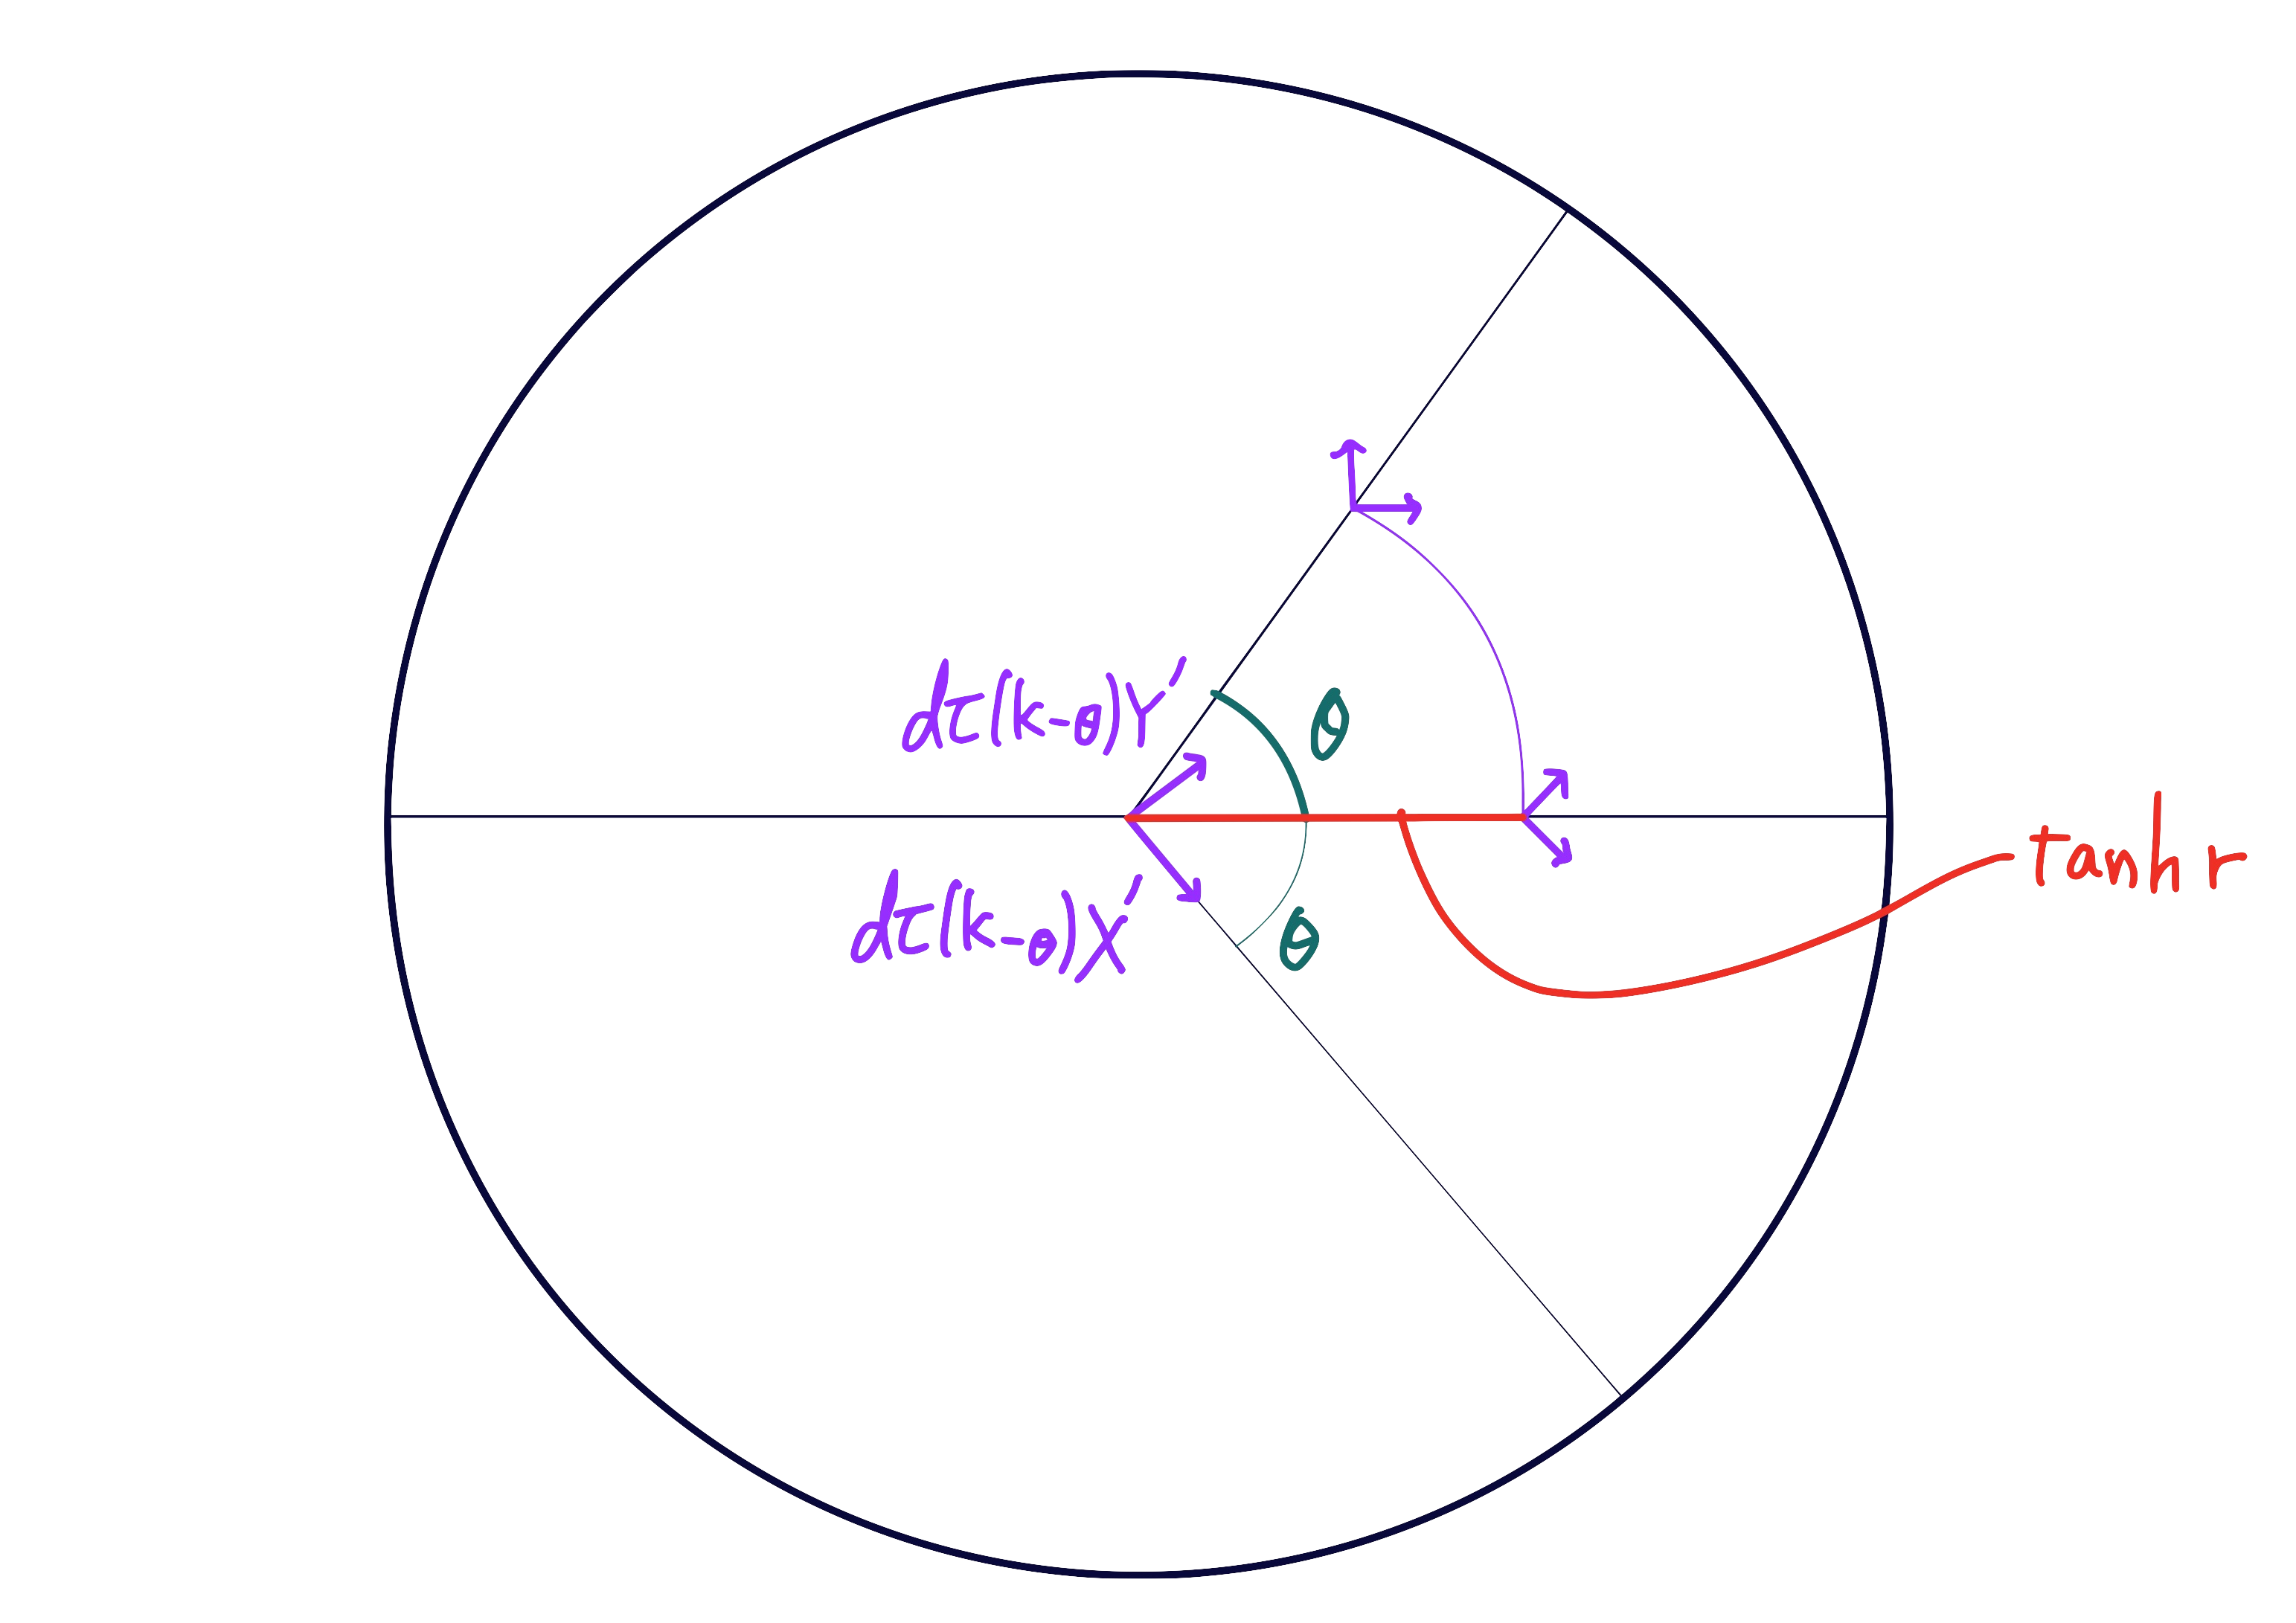
\includegraphics[scale=0.08]{../graph/riem-su11.png}
  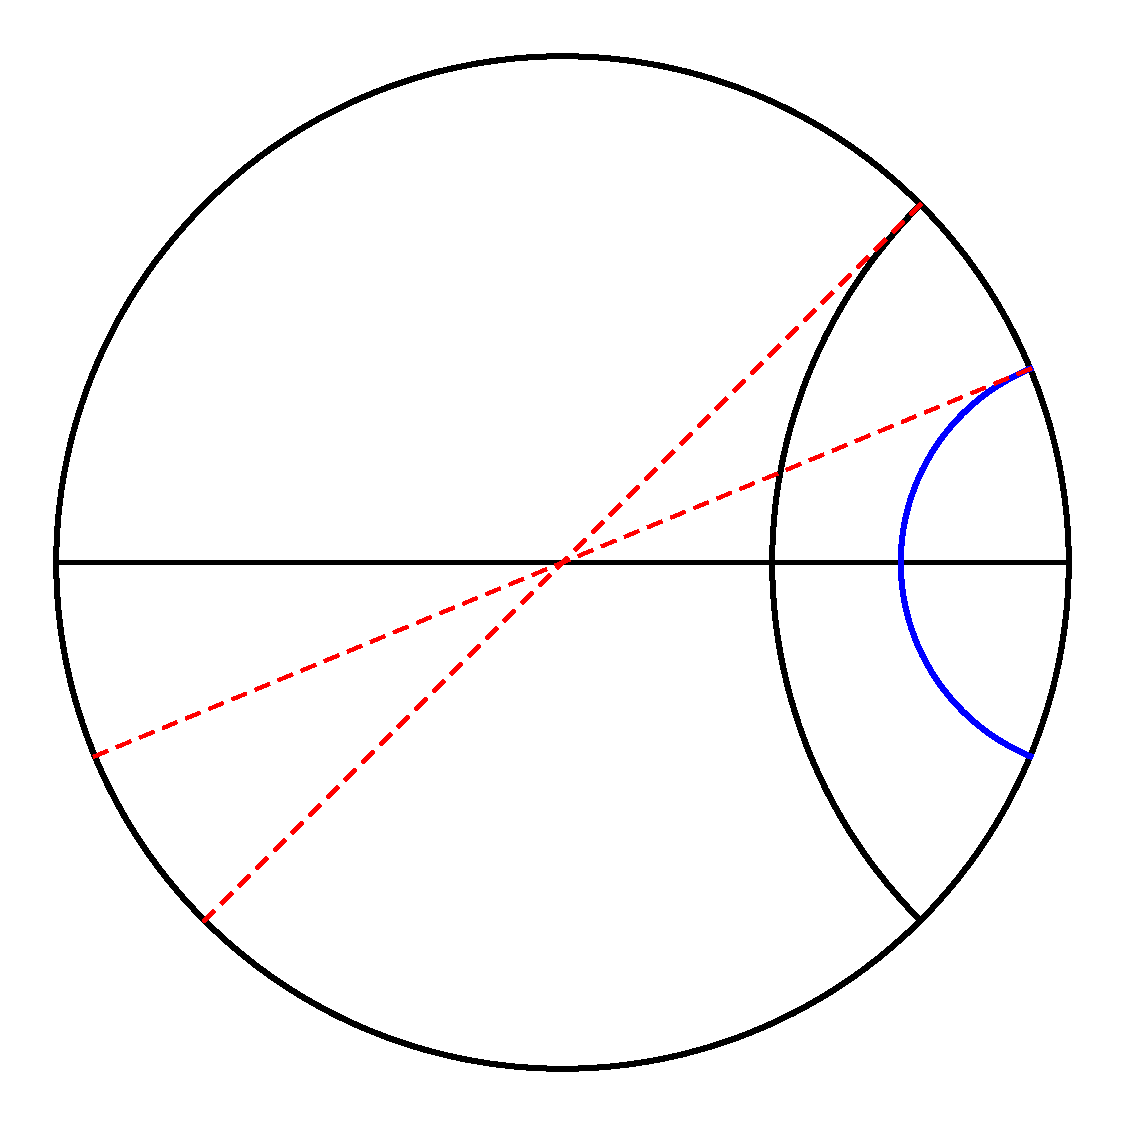
\includegraphics[scale=0.3]{../graph/visibility-2.pdf}
  \caption{visibility manifoldのイメージ}
  \label{fig:visibility}
\end{figure}


\begin{thm}({\cite[p.~296, 9.33~Theorem]{bh99}, originally \cite[Theorem~4.1]{e72-2}})\label{thm:visibility-and-rank}  
  $\exists C\cptsub M\st M = \bigcup\{f(C)\mid f\in \isom(M) \}  $なるHadamard多様体$M$に対し,次は同値である.
  \vspace{-1em}
  \begin{enumerate}
    \renewcommand{\labelenumi}{(\roman{enumi})}
  \item $M$はvisibility manifoldである.
  \item 全測地的な部分Riemann多様体$M'\subset M$で$\real^2$と等長同型なものが存在しない.
  \end{enumerate}
\end{thm}

ここでRiemann対称空間はHadamard多様体であり,\Cref{thm:visibility-and-rank}の (ii) は$G$の実階数が1以下であることと同値である.したがって$G$の実階数が1の場合$G/K$はvisibility manifoldであり,$G = \SU(1,2) $,$H= \SO(1,1)$の場合の証明と全く同様にして背理法により\Cref{prob:1121}が示される.

\subsection{$G$が実階数1の実半単純Lie群の直積の場合}
\Cref{thm:1216-main}の系として次が示される.
\begin{cor}\label{cor:0113-main}
  $n\in \nat$を固定し,$\{G_i \}_{1\leq i\leq n} $を実階数1の実線型半単純Lie群の族,$\Theta_i $を$G_i$のCartan対合とする.$G$を$\{G_i \}_{1\leq i\leq n} $の直積からなるLie群$G = G_1\times \cdots \times G_n $とし,$H = H_1\times \cdots \times H_n $を$G$の非コンパクトな閉部分群で$\Theta_i H_i = H_i$かつ$\dim \ha_i \cap\pe_i = 1$なるものとする.このとき$X\in \pe_{H,\bdd} $と任意の$1\leq i\leq n$に対して$X$の$\ge_i$への射影$X^{(i)}\in \ge_{i}$に対し$X^{(i)} \in \{0\}\cup\pe_i\setminus\ha_i $なることは同値である.
\end{cor}

% このとき$H_i\defeq G_i\cap H$とすると,$H \simeq H_1\times\cdots  \times H_n  $である.同様に$\ge_i\subset \ge = \bigoplus_{1\leq i\leq n}\ge_i $とみなすと$\ha_i\defeq \ge_i\cap \ha $は$H_i$のLie環である.

  
\begin{npfwn}[\Cref{cor:0113-main}]  
  各$G_i $を$G$の閉部分群と自然にみなす.$K_i$を$\Theta K_i = K_i $なる$G_i$の極大コンパクト部分群とすると,$K \defeq K_1\times \cdots \times K_n $は$G$の極大コンパクト部分群で,$\{\Theta_i\}_{1\leq i\leq n} $と整合的な$G$のCartan対合$\Theta$に対して$\Theta K = K $を満たす.

  $G/K\simeq G_1/K_1\times \cdots \times G_n/K_n $であり,\Cref{thm:kob89-lem6.1}により各$1\leq i\leq n$の$(G_i, H_i, G_i/K_i) $に対し上への微分同相$\pi_i\colon  (\ha_i\cap\pe_i)\oplus (\per{\ha_i}\cap \pe_i) \ni (Y_i, Z_i)\mapsto e^{Y_i}e^{Z_i}\cdot o_K \in G_i/K_i $が存在する.$X_i\in \pe_i $に対し$(Y_i(X_i), Z_i(X_i))\defeq \inv{\pi_i}(e^{X_i}K_i) $と定める.

  $X\in \pe$に対し,$X = X^{(1)} +\cdots + X^{(n)} $を$\pe = \bigoplus_{1\leq i\leq n}\pe_i $に対応する$X$の分解とすると,$Y(\real X) $が有界であることは各$Y_i(\real X^{(i)}) $が有界であることと同値である.また\Cref{thm:1216-main}より$Y_i(\real X^{(i)}) $が有界であることと$[X_1^{(i)}, X_2^{(i)} ] \neq 0 $あるいは$X^{(i)}_1 = 0 $であることが同値である.ここで$X^{(i)} =  X_1^{(i)} + X_2^{(i)}$は$\pe_i = (\ha_i\cap\pe_i)\oplus (\per{\ha_i}\cap\pe_i) $に対応する$X^{(i)}\in \pe_i $の分解とする.

  各$G_i$は実階数1であるから,上の条件は$X^{(i)}\in \{0\}\cup\pe_i\setminus\ha_i $と同値であり,\Cref{cor:0113-main}が示された.
\end{npfwn}


  % したがって,$Y(\real X) $が非有界であることと$[X_1, X_2] = 0 $かつ$X_1 \neq 0 $であることが同値であり,これは$X\in \ha\setminus\{0\} $と同値であるから\Cref{cor:0113-main}が示された.  


\begin{thebibliography}{99}
  \addcontentsline{toc}{section}{参考文献}
  % \bibitem[Benoist 09]{benoist-five-lectures} Y. Benoist, \textit{Five lectures on lattices in semisimple Lie groups}, S\'emin. Congr., Tome 18, 2009, pp. 117--76, Retrieved July 24, 2020 from \url{https://www.imo.universite-paris-saclay.fr/~benoist/prepubli/04lattice.pdf}\footnote{正式に出版された版 \url{https://smf.emath.fr/publications/cinq-cours-sur-les-reseaux-des-groupes-de-lie-semisimples} には大学経由でもアクセスできませんでした.}
\bibitem[Ber88]{ber88} J. N. Bernstein, \textit{On the support of Plancherel measure}, J. Geom. Phys., \textbf{5}, (1988), 663--710.
  % \bibitem[Bernstein--Reznikov]{ber-rez} J. Bernstein and A. Reznikov, \textit{Analytic continuation of representations and estimates of automorphic forms}, Ann. of Math. (2), Vol. 150, Issue 1, 1999, pp. 329--52
  % \bibitem[Borel]{borel276} A. Borel, Repr\'esentations de groupes localement compacts, Lecture Notes in Mathematics 276, Springer, 1972
\bibitem[BBE85]{bbe85} W. Ballmann, M. Brin and P. Eberlein, \textit{Structure of manifolds of nonpositive curvature. I}, Ann. of Math. (2),  \textbf{122}, (1985), 171--203.
\bibitem[BH99]{bh99} M.~R.~Bridson and A.~Haefliger, Metric Spaces of Non-Positive Curvature, Grundlehren der mathematischen Wissensschaften, Vol.~319, Springer-Verlag Berlin Heidelberg, 1999.
\bibitem[Borel--Ji]{borel-ji} A. Borel and L. Ji, Compactifications of Symmetric and Locally Symmetric Spaces, Mathematics: Theory \& Applications,  Birkhäuser  Boston, 2006.
  % \bibitem[Bourbaki Int. 7 et 8]{bour-int-7-and-8} N. Bourbaki, Int\'egration, Chaptires 7 et 8, \'El\'ements de math\'ematique, Springer, 2007
  % \bibitem[Bruhat 56]{bruhat56} F. Bruhat, \textit{Sur les repr\'esentations induites des groupes de Lie}, Bull. Soc. Math. France, \textbf{84}, 1956, pp. 97--205
  % \bibitem[Casselman]{casselman-dix-mal} William (Bill) Casselman, Essays on representations of real groups---The theorem of Dixmier \& Malliavin, Last revised January 24, 2016, Retrieved March 5, 2020 from \url{https://www.math.ubc.ca/~cass/research/pdf/Dixmier-Malliavin.pdf}
  % \bibitem[Conway]{conway} J. B. Conway, A Course in Functional Analysis---Second Edition, GTM 96, Springer, 2007
  % \bibitem[Dieudonn\'e]{dieudonne} J. Dieudonn\'e, Fundations of modern analysis---enlarged and corrected printing, international edition, Academic Press, 1969
\bibitem[Ebe72a]{e72-1} P.~Eberlien, \textit{Geodesic Flows on Negatively Curved Manifolds I}, Ann.~of~Math.~(2), \textbf{95}, (1972), 492--510.
\bibitem[Ebe72b]{e72-2} P.~Eberlien, \textit{Geodesic Flow in Certain Manifolds without Conjugate Points}, Trans.~Amer.~Math.~Soc., \textbf{167}, (1972), 151--70.
\bibitem[EO73]{eo73} P. Eberlein and B. O'Neill, \textit{Visibility Manifolds}, Pacific J. Math., \textbf{46}, (1973), 45--109.
  % \bibitem[Gromov \& Pansu]{gro-pan} M. Gromov and P. Pansu, \textit{Rigidity of lattices: An introduction}, In: P. de Bartolomeis and F. Tricerri eds., Geometric Topology: Recent Developments, Lecture Notes in Mathematics, vol. 1504, Springer, 1991
  % \bibitem[Halmos]{halmos} Paul. R. Halmos, Measure Theory, GTM 18, Springer, 1974
\bibitem[Hel84]{hel84} S. Helgason, Groups and Geometric Analysis---Integral Geometry, Invariant Differential Operators, and Spherical Functions, Mathematical Surveys and Monographs, Vol. 83, American Mathematical Society Province, Rhode Island, 1984.
\bibitem[Hel01]{hel01} S. Helgason, Differential Geometry, Lie Groups, and Symmetric Spaces, Graduate Studies in Mathematics, Vol. 34, American Mathematical Society, 2001.
  % \bibitem[Jenkins 73]{jenkins73} J. W. Jenkins, \textit{Growth of connected locally compact groups}, J. Funct. Anal., Vol. 12, Issue 1, 1973, pp. 113--27
  % \bibitem[Kassel--Kobayashi 16]{kk16} F. Kassel and T. Kobayashi, \textit{{\Poincare} series for non-Riemannian locally symmetric spaces}, Adv. Math., Vol. 287, 2016, pp. 123--236
  % \bibitem[Knapp 96]{knapp-beyond} A. W. Knapp, Lie Groups Beyond an Introduction, Progress in Mathematics, Vol. 140, Birkhäuser, 1996
\bibitem[KK16]{kk16} F. Kassel and T. Kobayashi, \textit{{\Poincare} series for non-Riemannian locally symmetric spaces}, Adv. Math., \textbf{287}, (2016), 123--236.
\bibitem[Kob89]{kob89} T. Kobayashi, 
  \textit{Proper action on a homogeneous space of reductive type},
  Math. Ann., \textbf{285}, (1989), 249--263.  
  % \bibitem[Kobayashi 96]{kobayashi96} T. Kobayashi, \textit{Criterion for proper actions on homogeneous spaces of reductive groups}, J. Lie Theory, Vol. 6, 1996, pp. 147--63
\bibitem[小林95]{kobayashi95} 小林俊行,球等質多様体上の調和解析入門,第3回整数論サマースクール `等質空間と保型形式' 所収,佐藤文広 編,長野,(1995),22--41.
\bibitem[Kob97]{kob97} T. Kobayashi, \textit{Invariant mesures on homogeneous manifolds of reductive type}, J. Reine Angew. Math., \textbf{1997}, (1997), 37--54.

  % \bibitem[Kobayashi 07]{kobayashi07} T. Kobayashi, \textit{A generalized Cartan decomposition for the double coset space $(U(n_1)\times U(n_2)\times U(n_3))\backslash U(n)/(U(p)\times U(q)) $}, J. Math. Soc. Japan, Vol. 59, No. 3, 2007, pp. 669--691
\bibitem[小林--大島]{kando} 小林俊行・大島利雄,リー群と表現論,岩波書店,2005.
\bibitem[Lee18]{lee2018} J. M. Lee, Introduction to Riemannian Manifolds Second Edition, Graduate Texts Mathematics 176, Springer International Publishing AG, 2018.
  % \bibitem[Reed--Simon I]{reed-simon-1} M. Reed \& B. Simon, Methods of Modern Mathematical Physics---I: Functional Analysis, Academic Press, 1972
  % \bibitem[Sasaki 10]{sasaki10} A. Sasaki, \textit{A characterization of non-tube type Hermitian symmetric spaces by visible actions}, Geom. Dedicata, Vol. 145, 2010, pp. 151--8 
  % \bibitem[辰馬]{tatsuma} 辰馬伸彦,位相群の双対定理,紀伊國屋数学叢書 32,紀伊國屋書店,1994
  % \bibitem[Moore 68]{moore} R. T. Moore, Measurable, continuous and smooth vectors for semigroups and group representations, Mem. Amer. Math. Soc., no. 78, 1968
  % \bibitem[Morris 15]{morris} D. W. Morris, \textit{Introduction to Arithmetic Groups}, arXiv:math/0106063v6, Published by Deductive Press, 2015
  % \bibitem[Varadarajan]{varadarajan} V. S. Varadarajan, Lie Groups, Lie Algebras, and Their Representations, GTM 102, Springer, 1984
  % \bibitem[Wallach I]{wallach1} N. R. Wallach, Real Reductive Groups I, Pure and Applied Mathematics, Vol. 132, Academic Press, 1988
  % \bibitem[吉田]{yoshida} 吉田耕作,復刊 超函数論,共立出版,2009
\bibitem[Yos37]{yos37} K.~Yosida, \textit{A problem concerning the second fundamental theorem of Lie}, Proc.~Imp.~Acad., \textbf{13}, (1937), 152--155.
\bibitem[Yos38]{yos38} K.~Yosida, \textit{A Theorem concerning the Semi-Simple Lie Groups}, \\Tohoku~Mathematical~Journal, First Series, \textbf{44}, (1938), 81--84.

  %%% Local Variables:
  %%% mode: latex
  %%% TeX-master: "okuda-master-thesis"
  %%% End:

\end{thebibliography}

\end{document}
